\phantomsection
\chapter[Analyzing the Coronavirus Spike Protein]{Analyzing the Coronavirus Spike Protein\chapsubhead{with Chris Lee}}
\label{chapter:coronavirus}
\renewcommand{\chaptertitle}{Analyzing the Coronavirus Spike Protein}
\addcontentsline{cc}{chapter}{Chapter \thechapter} % Adds chapter number to table of contents

\FloatBarrier

%\begin{quote}
%\textit{One of the world's most important warning systems for a deadly new outbreak is a doctor's or nurse's recognition that some new disease is emerging and then sounding the alarm. It takes intelligence and courage to step up and say something like that, even in the best of circumstances.}
%
%\begin{flushright}---~Tom Inglesby\end{flushright}
%\end{quote}

\section{A Tale of Two Doctors}
\label{sec:coronavirus_introduction}
\phantomsection

\FloatBarrier
\phantomsection
\subsection{The world's fastest outbreak}

On February 21, 2003, a Chinese doctor named Liu Jianlun flew to Hong Kong to attend a wedding and checked into Room 911 of the Metropole Hotel. The next day, he became too ill to attend the wedding and was admitted to a hospital. Two weeks later, he was dead.

On his deathbed, Dr. Liu stated that he had recently treated sick patients in Guangdong Province, where a highly contagious respiratory illness had infected hundreds of people. The Chinese government had made brief mention of this incident to the World Health Organization (WHO) but had concluded that the likely culprit was a common bacterial infection. By the time anyone realized the severity of the disease, it was already too late to stop the outbreak.

On February 23, a man who had stayed across the hall from Dr. Liu at the Metropole traveled to Hanoi and died after infecting 80 people. On February 26, a woman checked out of the Metropole, traveled back to Toronto, and died after initiating an outbreak there. On March 1, a third guest was admitted to a hospital in Singapore, where sixteen additional cases of the illness arose within two weeks.

Consider that the Black Death, which killed over a third of all Europeans, took four years to travel from Constantinople to Kiev. Or that HIV took two decades to circle the globe. In contrast, this mysterious new disease had crossed the Pacific Ocean within a week of entering Hong Kong.

As health officials braced for the impact of the fastest traveling virus in human history, panic set in. Businesses were closed, sick passengers were removed from airplanes, and Chinese officials threatened to execute anyone deliberately spreading the disease. In the process, the mysterious new illness earned a name: \textdefnogloss{severe acute respiratory syndrome}, or \textdefnogloss{SARS}.

\FloatBarrier
\phantomsection
\subsection{Tracing the source of the outbreak}

SARS was deadly, killing close to 10\% of those who became sick. But it also struggled to spread within the human population, and it was contained in July 2003 after accumulating fewer than 10,000 confirmed symptomatic cases worldwide.

In 2017, researchers published the results of sampling horseshoe bats for five years in a cave in Yunnan province. They found that these bats harbored coronaviruses with remarkable genetic similarity to the virus causing SARS. Yet their work has become infamous because they identified additional coronaviruses in the bats that were capable of entering human cells. Their words are now chilling:

\begin{itquote}
We have also revealed that various \emph{[}viruses\emph{]}~\ldots~are still circulating among bats in this region. Thus, the risk of spillover into people and emergence of a disease similar to SARS is possible. This is particularly important given that the nearest village to the bat cave we surveyed is only 1.1 km away, which indicates a potential risk of exposure to bats for the local residents. Thus, we propose that monitoring of SARSr-CoV evolution at this and other sites should continue, as well as examination of human behavioral risk for infection and serological surveys of people, to determine if spillover is already occurring at these sites and to design intervention strategies to avoid future disease emergence.
\end{itquote}

\FloatBarrier
\phantomsection
\subsection{A new threat emerges}

On December 30, 2019, a Chinese ophthalmologist named Li Wenliang sent a WeChat message to fellow doctors at Wuhan Central Hospital, warning them that he had seen several patients with symptoms resembling SARS. He urged his colleagues to wear protective clothing and masks to shield them from this new threat.

The next day, a screenshot of his post was leaked online, and local police summoned Dr. Li and forced him to sign a statement that he had ``severely disturbed public order''. He then returned to work, treating patients in the same Wuhan hospital.

Meanwhile, WHO received reports of multiple pneumonia cases from the Wuhan Municipal Health Commission and activated a support team to assess the new disease. WHO declared on January 14 that local authorities had seen ``no clear evidence of human-to-human transmission of the novel coronavirus''. But once again, it was already too late.

Throughout January, the virus silently raged through China as Lunar New Year celebrations took place within the country, and it spread to both South Korea and the United States. By the end of the month, the disease was in 19 countries, becoming a pandemic and earning a name in the process: \textdefnogloss{coronavirus disease 2019 (COVID-19)}.

As for Dr. Li? Despite warning against the risk of the new virus, he contracted COVID-19 from one of his patients on January 8. He continued working until he was forced to be admitted to the hospital on January 31. Within a week, he was dead, one of the first of millions of COVID-19 casualties.\\

\FloatBarrier
\phantomsection
\section{Protein Sequence and Structure}

\FloatBarrier
\phantomsection
\subsection{The sequence of the SARS-CoV-2 spike protein}

The viruses causing the two outbreaks, \textdefnogloss{SARS coronavirus (SARS-CoV)} and \textdefnogloss{SARS coronavirus 2 (SARS-CoV-2)} are both \textdef{coronaviruses}{coronavirus}{a family of viruses whose outer membrines are covered in spike proteins, which cause them to look like the sun's corona during an eclipse}, which means that their outer membranes are covered in a layer of \textdef{spike proteins}{spike protein}{a protein covering the surface of a coronavirus that the virus uses to latch on to cells} that cause them to look like the sun's corona during an eclipse (\autoref{fig:coronavirus}).

\begin{figure}[h]
	\centering
	\mySfFamily
	\includegraphics[width = 0.6\textwidth]{../images/coronavirus.png}
	\caption{Coronaviruses as seen under a microscope. The fuzzy blobs on the cell surface are spike proteins, which the virus uses to gain entry to host cells.}
	\label{fig:coronavirus}
\end{figure}

When viewed under a microscope, the two viruses look identical, and they use the same mechanism to infect human cells, when the spike protein on the virus surface bonds to the ACE2 enzyme on a human cell's membrane. So why did SARS fizzle, but SARS-CoV-2, a disease that is on average less harmful and less deadly to individuals who contract it, transform into a pandemic? The most likely explanation for the ability of SARS-CoV-2 to spread across far more countries and remain a public health threat even in the face of lockdowns is that it spreads more easily; that is, it is more \textdefnogloss{infectious}. Is there a molecular basis of this increased infectiousness?

We will place ourselves in the shoes of early SARS-CoV-2 researchers studying the new virus in early 2020. The virus's genome, consisting of nearly 30,000 nucleotides, was published on January 10, and an annotation of this genome identifying the location of the virus's genes is shown in \autoref{fig:SARSCoV2Annotation}. Upon sequence comparison, SARS-CoV-2 was found to be related to several coronaviruses isolated from bats and distantly related to SARS-CoV.

\begin{figure}[h]
	\centering
	\mySfFamily
	\includegraphics[width = 0.85\textwidth]{../images/SARSCoV2Annotation.png}
	\caption{An annotated genome of SARS-CoV-2, with rectangles showing the location of areas encoding RNA or protein. The spike protein, found at the bottom of this image, is labeled ``S'' and begins at nucleotide position 21,563.}
	\label{fig:SARSCoV2Annotation}
\end{figure}

Recall from our discussion of transcription factors in \autoref{chapter:motifs} that by the central dogma of molecular biology, DNA is transcribed into RNA, which is then translated into protein. According to the genetic code, triplets of RNA nucleotides called codons are converted into single amino acids. The resulting chain of amino acids is called a \textdef{polypeptide}{polypeptide}{a linear chain of amino acids that forms part or all of a protein}.\\

\begin{note}[%
Coronaviruses are RNA viruses, which means that they do not have DNA and their genome is encoded as a single strand of RNA. As a result, they bypass the DNA to RNA transcription process.
]\end{note}

The gene encoding the spike protein starts at nucleotide position 21,563 of the SARS-CoV-2 genome, and the corresponding translated polypeptide chain is shown in \autoref{fig:spike_protein_sequence}. Each of the 20 standard amino acids is represented by a letter taken from the Latin alphabet (all letters except for ``B'', ``J'', ``O'', ``U'', ``X'', and ``Z'' are used). As you examine the string of letters in \autoref{fig:spike_protein_sequence}, consider how global mayhem can ultimately be caused by something so tiny.

\begin{figure}[h]
\begin{ttsequence}[0.93]MFVFLVLLPLVSSQCVNLTTRTQLPPAYTNSFTRGVYYPDKVFRSSVLHSTQDLFLPFFSNVTWFHAIHV\\
SGTNGTKRFDNPVLPFNDGVYFASTEKSNIIRGWIFGTTLDSKTQSLLIVNNATNVVIKVCEFQFCNDPF\\
LGVYYHKNNKSWMESEFRVYSSANNCTFEYVSQPFLMDLEGKQGNFKNLREFVFKNIDGYFKIYSKHTPI\\
NLVRDLPQGFSALEPLVDLPIGINITRFQTLLALHRSYLTPGDSSSGWTAGAAAYYVGYLQPRTFLLKYN\\
ENGTITDAVDCALDPLSETKCTLKSFTVEKGIYQTSNFRVQPTESIVRFPNITNLCPFGEVFNATRFASV\\
YAWNRKRISNCVADYSVLYNSASFSTFKCYGVSPTKLNDLCFTNVYADSFVIRGDEVRQIAPGQTGKIAD\\
YNYKLPDDFTGCVIAWNSNNLDSKVGGNYNYLYRLFRKSNLKPFERDISTEIYQAGSTPCNGVEGFNCYF\\
PLQSYGFQPTNGVGYQPYRVVVLSFELLHAPATVCGPKKSTNLVKNKCVNFNFNGLTGTGVLTESNKKFL\\
PFQQFGRDIADTTDAVRDPQTLEILDITPCSFGGVSVITPGTNTSNQVAVLYQDVNCTEVPVAIHADQLT\\
PTWRVYSTGSNVFQTRAGCLIGAEHVNNSYECDIPIGAGICASYQTQTNSPRRARSVASQSIIAYTMSLG\\
AENSVAYSNNSIAIPTNFTISVTTEILPVSMTKTSVDCTMYICGDSTECSNLLLQYGSFCTQLNRALTGI\\
AVEQDKNTQEVFAQVKQIYKTPPIKDFGGFNFSQILPDPSKPSKRSFIEDLLFNKVTLADAGFIKQYGDC\\
LGDIAARDLICAQKFNGLTVLPPLLTDEMIAQYTSALLAGTITSGWTFGAGAALQIPFAMQMAYRFNGIG\\
VTQNVLYENQKLIANQFNSAIGKIQDSLSSTASALGKLQDVVNQNAQALNTLVKQLSSNFGAISSVLNDI\\
LSRLDKVEAEVQIDRLITGRLQSLQTYVTQQLIRAAEIRASANLAATKMSECVLGQSKRVDFCGKGYHLM\\
SFPQSAPHGVVFLHVTYVPAQEKNFTTAPAICHDGKAHFPREGVFVSNGTHWFVTQRNFYEPQIITTDNT\\
FVSGNCDVVIGIVNNTVYDPLQPELDSFKEELDKYFKNHTSPDVDLGDISGINASVVNIQKEIDRLNEVA\\
KNLNESLIDLQELGKYEQYIKWPWYIWLGFIAGLIAIVMVTIMLCCMTSCCSCLKGCCSCGSCCKFDEDD\\
SEPVLKGVKLHYT\phantom{QCVNLTTRTQLPPAYTNSFTRGVYYPDKVFRSSVLHSTQDLFLPFFSNVTWFHAIHV}
\end{ttsequence}
\caption{The 1,273 amino acid sequence of the SARS-CoV-2 spike protein. Each symbol represents one of 20 amino acids.}
\label{fig:spike_protein_sequence}
\end{figure}

\phantomsection
\subsection{Nature's magic protein folding algorithm}

After the SARS-CoV-2 spike protein polypeptide chain is formed, it will ``fold'' into a three-dimensional shape. This folding process occurs spontaneously for all proteins and without any outside influence, and the same polypeptide chain will almost always fold into the same 3-D structure in a manner of microseconds. Nature must be applying some ``magic algorithm'' to quickly produce the folded structure of a protein from its sequence of amino acids.

Predicting the folded structure of a polypeptide is called \textdef{protein structure prediction}{protein structure prediction}{the problem of predicting the folded three-dimensional structure of a polypeptide from its nucleotide sequence}, a problem that is simple to state but difficult to solve. In fact, protein structure prediction has been an active area of biological research for several decades.

Why do we care about protein structure? Knowing a protein's structure is essential to determining its function and how it interacts with other proteins or molecules in its environment. After all, we still do not know the function of a few thousand human genes, and \autoref{fig:different_protein_shapes_2020} shows the huge variety of protein shapes in the 2020 ``proteins of the month'' named by the \textdef{Protein Data Bank (PDB)}{Protein Data Bank (PDB)}{a public database for the structural study of proteins}. (Note that the June 2020 winner is the SARS-CoV-2 spike protein.)

\begin{figure}[h]
	\centering
	\mySfFamily
	\includegraphics[width = 0.85\textwidth]{../images/different_protein_shapes_2020.jpg}
	\caption{Each ``molecule of the month'' in 2020 named by the PDB. These proteins have widely varying shapes and accomplish a wide variety of cellular tasks. The SARS-CoV-2 spike protein was the molecule of the month in June.}
	\label{fig:different_protein_shapes_2020}
\end{figure}

Another central problem in protein structural research is devoted to understanding protein interactions. For example, a disease may be caused by a faulty protein, in which case researchers want to find a drug that binds to the protein and causes some change of interest in that protein, such as inhibiting its behavior.

In our work with SARS-CoV-2 spike protein analysis, we will consider two questions. First, can we reverse engineer nature's magic algorithm and determine the spike protein's shape from its sequence of amino acids in \autoref{fig:spike_protein_sequence}? Second, once we know this molecular structure of the SARS-CoV-2 spike protein, how does its structure and function differ from the same protein in SARS-CoV?\\

\FloatBarrier
\phantomsection

\section{Protein Structure Prediction is Difficult}
\label{sec:structure_intro}

\phantomsection
\subsection{Experimental methods for determining protein structure}

Although we would like to infer nature's magic algorithm for inferring protein structure from amino acid sequence, biochemists can determine the structure of a protein experimentally. In \textdef{X-ray crystallography}{X-ray crystallography}{an experimental process in which researchers crystallize many copies of a molecule such as a protein and then shine an intense beam of X-rays at the crystal in order to determine the molecule's structure}, researchers crystallize many copies of a protein and then shine an intense beam of X-rays at the crystal. The light hitting the protein is diffracted, creating patterns from which the position of every atom in the protein can be inferred.

X-ray crystallography is over a century old and has been the \textit{de facto} approach for protein structure determination for decades. Yet a newer method is now rapidly replacing X-ray crystallography. In \textdef{cryo-electron microscopy (cryo-EM)}{cryo-electron microscopy (cryo-EM)}{an experimental process in which researchers preserve thousands of copies of a molecule such as a protein in non-crystalline ice and then examine these copies with an electron microscope}, researchers preserve thousands of copies of a protein in non-crystalline ice and then examine these copies with an electron microscope.

Unfortunately, laboratory approaches for structure determination are expensive and cannot be used on all proteins. An X-ray crystallography experiment for a single protein costs upward of \$2,000, and building an electron microscope can cost millions. When applying X-ray crystallography, crystallizing a protein is a challenging task, and each copy of the protein must line up in the same way, which does not work for very flexible proteins.  And to study bacterial proteins, we need to culture the bacteria in the lab, but microbiologists have estimated that fewer than 2\% of bacteria can be cultured with current approaches.

Protein structures that have been determined experimentally are typically stored in the PDB, which contains over 160,000 protein structures. This number may seem large, but a recent study estimated that the 20,000 human genes translate into between 620,000 and 6.13 million protein isoforms (i.e., protein variants with slightly different structures). If we hope to catalog the proteins of all living things, then our work on structure determination is just beginning.

\FloatBarrier
\phantomsection
\subsection{Protein sequence and structure do not correlate well}

The prediction of protein structure from amino acid sequence is challenging because this prediction is fine-tuned with respect to some mutations but robust with respect to others. On the one hand, small perturbations in a protein's sequence can drastically change the protein's shape and even render it useless. On the other hand, different amino acids can have similar chemical properties, and so some sequence mutations will hardly change the structure of the protein. As a result, two very different amino acid sequences can fold into proteins with similar structure and comparable function.

Continuing with our hemoglobin example, \autoref{fig:SequenceStructureExample} compares the sequences and structures of hemoglobin subunit alpha taken from three species: humans, shortfin mako sharks, and emus. Hemoglobin is the oxygen-transport protein in the blood, consisting of two alpha ``subunit'' proteins and two beta subunit proteins that combine into a protein complex; because hemoglobin is well-studied and much shorter than the SARS-CoV-2 spike protein (the alpha and beta subunits are only 140 and 146 amino acids long, respectively), we will use it as an example throughout this chapter. The alpha subunits for the three species are markedly different in terms of amino acid sequence, and yet their structures are essentially identical.\\

\begin{figure}[h]
	\centering
	\mySfFamily
	\includegraphics[width = 0.85\textwidth]{../images/SequenceStructureExample.png}
	\caption{(Top) An amino acid sequence comparison of the first 40 (out of 140) amino acids of hemoglobin subunit alpha for three species: human (PDB entry: \href{https://www.rcsb.org/structure/1si4}{1si4}), shortfin mako shark (PDB entry: \href{https://www.rcsb.org/structure/3mkb}{3mkb}), and emu (PDB entry: \href{https://www.rcsb.org/structure/3wtg}{3wtg}). A column is colored blue if all three species have the same amino acid, white if two species have the same amino acid, and red if all amino acids are different. Sequence identity calculates the number of positions in two amino acid sequences that share the same amino acid. (Bottom) Side by side comparisons of the 3-D structures of the three proteins. The final figure on the right superimposes the first three structures to highlight that they are virtually identical.}
	\label{fig:SequenceStructureExample}
\end{figure}

\phantomsection
\subsection{Flexible polypeptide chains can fold into many possible structures}

Another reason why protein structure prediction is so difficult is because a polypeptide is very flexible, with the ability to rotate in multiple ways at each amino acid, which means that the polypeptide can fold into a staggering number of different shapes. This polypeptide flexibility owes to the molecular structure of amino acids.

As shown in \autoref{fig:AminoAcid}, an amino acid comprises four parts. In the center, a carbon atom (called the \textdef{alpha carbon}{alpha carbon}{the central carbon atom of an amino acid}) is connected to four different molecules: a hydrogen atom (H), a \textdefnogloss{carboxyl group} ($-\text{COOH}$), an \textdefnogloss{amino group} ($-\text{NH}_2$), and a \textdefnogloss{side chain} (denoted ``R'' and often called an \textbf{R group}). The side chain is a molecule that differs between different amino acids and ranges in mass from a single hydrogen atom (glycine) up to $-\text{C}_8\text{H}_7\text{N}$ (tryptophan).

\begin{figure}[h]
	\centering
	\mySfFamily
	\includegraphics[width = 0.4\textwidth]{../images/AminoAcid.png}
	\caption{An amino acid consists of a central, alpha carbon attached to a hydrogen atom, a side group, a carboxyl group, and an amino group.}
	\label{fig:AminoAcid}
\end{figure}

To form a polypeptide chain, consecutive amino acids are linked together during a condensation reaction in which the amino group of one amino acid is joined to the carboxyl group of another, while a water molecule ($\text{H}_2\text{O}$) is expelled (\autoref{fig:condensation} (top)). The resulting bond that is produced between the carbon atom of one amino acid's carboxyl group and the nitrogen atom of the next amino acid's amino group, called a \textdefnogloss{peptide bond}, is very strong. The peptide has very little rotation around this bond, which is almost always locked at 180\textdegree. As peptide bonds are formed between adjacent amino acids, the polypeptide chain takes shape (\autoref{fig:condensation} (bottom)).

\begin{figure}[h]
	\centering
	\mySfFamily
	\includegraphics[width = 0.85\textwidth]{../images/dipeptide_reaction.png}\\[0.5ex]
	\includegraphics[width = 0.6\textwidth]{../images/Backbone.png}
	\caption{(Top) A condensation reaction joins two amino acids into a ``dipeptide'' by joining the amino group of one amino acid to the carboxyl group of the other, with a water molecule expelled. (Bottom) A polypeptide chain formed of three amino acids.}
	\label{fig:condensation}
\end{figure}

However, the bonds \textit{within} an amino acid, joining the alpha carbon to its carboxyl group and amino group, are not as rigid, and the polypeptide is free to rotate around these two bonds. This rotation produces two angles of interest, called the \textdefnogloss{phi angle} ($\phi$) and \textdefnogloss{psi angle} ($\psi$) (\autoref{fig:torsion_angles}), which are formed at the alpha carbon's connections to its amino group and carboxyl group, respectively.\\

\begin{figure}[h]
	\centering
	\mySfFamily
	\includegraphics[width = 0.25\textwidth]{../images/torsion_angles.png}
	\caption{A polypeptide chain of multiple amino acids with the torsion angles $\phi$ and $\psi$ indicated. The angle ω indicates the angle of the peptide bond, which is typically 180\textdegree.}
	\label{fig:torsion_angles}
\end{figure}

A good analogy for polypeptide flexibility is the ``Rubik's Twist'' puzzle, which consists of a linear chain of flexible blocks that can form many different shapes. \autoref{fig:rubiks_twist_four_panel} shows the Rubik's Twist folding into a ball.

\begin{figure}[h]
	\centering
	\mySfFamily
	\includegraphics[width = 0.75\textwidth]{../images/rubiks_twist_four_panel.jpg}
	\caption{Each section of the Rubik's Twist puzzle can be rotated, allowing the toy to take on many different conformations, such as a ball (bottom right).}
	\label{fig:rubiks_twist_four_panel}
\end{figure}

A polypeptide with \textit{n} amino acids has $n - 1$ peptide bonds, meaning that its shape is influenced by $n - 1$ phi angles and $n - 1$ psi angles. If each bond angle has \textit{k} possible values, then the polypeptide has $k^{2n-2}$ total possible conformations. If \textit{k} is equal to 3 and \textit{n} is equal to only 100 (representing a short polypeptide), then the number of potential protein structures is more than the number of atoms in the universe! The ability of the magic algorithm to reliably find a single conformation despite such an enormous number of potential shapes is called \textdef{Levinthal's paradox}{Levinthal's paradox}{the conundrum that a protein reliably folds into a single conformation despite there being an enormous number of potential structures for that protein}.

Although protein structure prediction is difficult, it is not impossible; the magic algorithm is not, after all, magic. But before discussing how we can solve this problem, we will need to learn a few more biochemical details and be more precise about two things. First, we should specify what we mean by the ``structure'' of a protein. Second, although we know that a polypeptide always folds into the same final three-dimensional shape, we have not said anything about \textit{why} a protein folds in a certain way. We will therefore need a better understanding of how the physicochemical properties of amino acids influence a protein's final structure.\\

\FloatBarrier
\phantomsection

\section{Protein Biochemistry}

\FloatBarrier
\phantomsection
\subsection{The four levels of protein structure}

Protein structure is a broad term that encapsulates four different levels of description. A protein's \textdef{primary structure}{primary structure}{the amino acid sequence of a polypeptide chain} refers to the amino acid sequence of the polypeptide chain, which we saw in \autoref{fig:spike_protein_sequence} for the SARS-CoV-2 spike protein.

A protein's \textdef{secondary structure}{secondary structure}{the highly regular, repeating intermediate substructures of a protein that form before the overall protein folding process completes} describes its highly regular, repeating intermediate substructures that form before the overall protein folding process completes. The two most common such substructures, shown in \autoref{fig:hemoglobin_secondary_structure}, are \textdef{alpha helices}{alpha helix}{a protein secondary structure that occurs when nearby amino acids wrap around to form a tube structure} and \textdef{beta sheets}{beta sheet}{a protein secondary structure that occurs when nearby amino acids line up side-by-side}. Alpha helices occur when nearby amino acids wrap around to form a tube structure; beta sheets occur when nearby amino acids line up side-by-side.\\

\begin{figure}[h]
	\centering
	\mySfFamily
	\includegraphics[width = 0.85\textwidth]{../images/hemoglobin_secondary_structure.png}
	\caption{The general shape of alpha helices (left) and beta sheets (right), the two most common protein secondary structures.}
	\label{fig:hemoglobin_secondary_structure}
\end{figure}

A protein's \textdef{tertiary structure}{tertiary structure}{the final, stable 3D shape of a protein's polypeptide chain} describes its final 3D shape after the polypeptide chain has folded and is chemically stable. Throughout this chapter, when discussing the ``shape'' or ``structure'' of a protein, we are almost exclusively referring to its tertiary structure. \autoref{fig:hemoglobin_tertiary_structure} shows the tertiary structure of human hemoglobin subunit alpha. For the sake of simplicity, this figure does not show the position of every atom in the protein but rather represents the protein shape as a composition of secondary structures.\\

\begin{figure}[h]
	\centering
	\mySfFamily
	\includegraphics[width = 0.7\textwidth]{../images/hemoglobin_tertiary_structure.png}
	\caption{The tertiary structure of human hemoglobin subunit alpha. Within the structure are multiple alpha helix secondary structures.}
	\label{fig:hemoglobin_tertiary_structure}
\end{figure}

Finally, some proteins have a \textdef{quaternary structure}{quaternary structure}{the arrangement of a protein's subunits with respect to each other to form a single functional unit}, which describes the protein’s interaction with other copies of itself to form a single functional unit, or a \textdef{multimer}{multimer}{a protein formed of more than one polypeptide chain}. Many proteins do not have a quaternary structure and function as an independent monomer. \autoref{fig:quaternary_structure} (left) shows the quaternary structure of hemoglobin, which is a multimer consisting of two alpha subunits and two beta subunits.

As for coronaviruses, the spike protein is a \textdefnogloss{homotrimer}, meaning that it is formed of three essentially identical units called \textdef{chains}{chain}{a subunit of a multimer}, each one translated from the corresponding region of the coronavirus's genome; these chains are colored differently in \autoref{fig:quaternary_structure} (right). In this chapter, when discussing the structure of the spike protein, we often are referring to the structure of a single chain.\\

\begin{figure}[h]
	\centering
	\mySfFamily
	\tabcolsep = 1em
	\begin{tabular}{c c}
	\includegraphics[width = 0.35\textwidth]{../images/hemoglobin_quaternary_structure.png} & \includegraphics[width = 0.45\textwidth]{../images/spike_protein_homotrimer.png}
	\end{tabular}
	\caption{(Left) The quaternary structure of human hemoglobin, which consists of two alpha subunits (shown in red) and two beta subunits (shown in blue). Each alpha subunit is the tertiary structure from \autoref{fig:hemoglobin_tertiary_structure}. (Right) A side and top view of the quaternary structure of the SARS-CoV-2 spike protein homotrimer, with its three chains highlighted using different colors.}
	\label{fig:quaternary_structure}
\end{figure}

The structural units making up proteins are often hierarchical, and the spike protein is no exception. Each spike protein chain is a \textdefnogloss{dimer}, consisting of two subunits called \textdefnogloss{S1} and \textdefnogloss{S2}. Each of these subunits further divides into \textdef{protein domains}{protein domain}{a distinct structural unit within a protein that folds independently and is typically responsible for a specific interaction or function}, distinct structural units within the protein that fold independently and are typically responsible for a specific interaction or function. For example, the SARS-CoV-2 spike protein has a \textdefnogloss{receptor binding domain (RBD)} located on the S1 subunit of the spike protein that is responsible for interacting with the human ACE2 enzyme; the rest of the protein does not come into contact with ACE2. We will say more about the RBD soon.

\FloatBarrier
\subsection{Proteins seek the lowest energy conformation}

Now that we know a bit more about how protein structure is defined, we will discuss why proteins fold in the same every time. In other words, what are the factors driving the magic algorithm?

Amino acids' side chain variety causes them to have different chemical properties, which can lead to some protein conformations being more chemically ``preferable'' than others. For example, \autoref{fig:AminoAcidChart} groups the twenty amino acids commonly occurring in proteins according to their chemical properties. Nine of these amino acids are \textdefnogloss{hydrophobic} (also called \textdefnogloss{nonpolar}), meaning that their side chains are repelled by water, and so we tend to find these amino acids tucked away on the interior of the protein.

\begin{figure}[h]
	\centering
	\mySfFamily
	\includegraphics[width = 0.85\textwidth]{../images/AminoAcidChart.png}
	\caption{A chart of the twenty amino acid grouped by chemical properties. The side chain of each amino acid is highlighted in blue.}
	\label{fig:AminoAcidChart}
\end{figure}

We can therefore view protein folding as finding the tertiary structure that is the most \textit{stable} given a polypeptide's primary structure. A central theme of \autoref{chapter:chemotaxis} was that a system of chemical reactions moves toward equilibrium. The same principle is true of protein folding; when a protein folds into its final structure, it reaches a conformation that is as chemically stable as possible.

To be more precise, the \textdef{potential energy}{potential energy}{the energy stored within a molecule due to its position, state, and arrangement, sometimes called free energy} (sometimes called \textdefnogloss{free energy}) of a molecule is the energy stored within an object due to its position, state, and arrangement. In molecular mechanics, the potential energy is made up of the sum of \textdef{bonded energy}{bonded energy}{the potential energy of a molecule deriving from the molecule's covalent bonds} and \textdef{non-bonded energy}{non-bonded energy}{the potential energy of a molecule deriving from electrostatic interactions and van der Waals interactions}.

As the protein bends and twists into a stable conformation, bonded energy derives from the protein's covalent bonds, as well as the bond angles between adjacent amino acids, and the torsion angles that we introduced earlier.

Non-bonded energy comprises \textdef{electrostatic interactions}{electrostatic interactions}{attraction and repulsion forces from electric charge between charged amino acids} and \textdef{van der Waals interactions}{van der Waals interactions}{interactions between nearby atoms due to random imbalances in the locations of electrons}. Electrostatic interactions refer to the attraction and repulsion forces from the electric charge between pairs of charged amino acids. Two of the twenty standard amino acids (arginine and lysine) are positively charged, and two (aspartic acid and glutamic acid) are negatively charged. Two nearby amino acids of opposite charge may interact to form a \textdef{salt bridge}{salt bridge}{an interaction between two nearby amino acids in a protein of opposite charge}. Conformations that contain salt bridges and keep apart similarly charged amino acids will therefore have a lower free energy component contributed by electrostatic interactions.

As for van der Waals interactions, atoms are dynamic systems, with electrons constantly buzzing around the nucleus. However, due to random chance, the negatively charged electrons in an atom could momentarily be unevenly distributed on one side of the nucleus. This uneven distribution will cause the atom to have a temporary negative charge on the side with the excess electrons and a temporary positive charge on the opposite side. As a result of this charge, one side of the atom may attract only the oppositely charged components of another atom, creating an \textdefnogloss{induced dipole} in that atom (\autoref{fig:van_der_waals}). Van der Waals forces refer to the attraction and repulsion between atoms because of induced dipoles.

%\begin{figure}[h]
%	\centering
%	\mySfFamily
%	\includegraphics[width = 0.4\textwidth]{../images/van_der_waals_normal.png}
%	\caption{A carbon-12 atom showing six positively charged protons (green), six neutrally charged neutrons (blue), and six negatively charged electrons (red). Under typical circumstances, the electrons will most likely be distributed uniformly around the nucleus.}
%	\label{fig:van_der_waals_normal}
%\end{figure}

\begin{figure}[h]
	\centering
	\mySfFamily
	\includegraphics[width = 0.85\textwidth]{../images/van_der_waals.png}
	\caption{Due to random chance, the electrons in the atom on the left have clustered on the left side of the atom, creating a net negative charge on this side of the atom, and therefore a net positive charge on the right side of the atom. This polarity induces a dipole in the atom on the right, whose electrons are attracted because of van der Waals forces.}
	\label{fig:van_der_waals}
\end{figure}

As the protein folds, it seeks a conformation of \textit{lowest} total potential energy based on the combination of all the above-mentioned forces. For an analogy, imagine a ball on a slope (\autoref{fig:EnergyCartoon}). The ball will move down the slope unless it is pushed uphill by some outside force, making it unlikely that the ball will wind up at the top of a hill. We will keep this analogy in mind as we return to the problem of protein structure prediction.\\

\begin{figure}[h]
	\centering
	\mySfFamily
	\includegraphics[width = 0.65\textwidth]{../images/EnergyCartoon.png}
	\caption{A ball on a slope offers an analogy for a protein folding into the lowest energy structure. As the ball is more likely to move down into a valley, a protein is more likely to fold into a more stable, lower energy conformation.}
	\label{fig:EnergyCartoon}
\end{figure}

\FloatBarrier
\phantomsection

\section{\textit{Ab initio} Protein Structure Prediction}
\label{sec:ab_initio}

\phantomsection
\subsection{Modeling \textit{ab initio} structure prediction as an exploration problem}

Predicting a protein’s structure using only its amino acid sequence is called \textdef{\textit{ab initio} structure prediction}{ab initio structure prediction}{the prediction of a protein's structure using only its amino acid sequence} (\textit{ab initio} means “from the beginning” in Latin). Although many different algorithms have been developed for \textit{ab initio} protein structure over the years, these algorithms all find themselves solving a similar problem.

Biochemical research has contributed to the development of scoring functions called \textdef{force fields}{force field}{an approach that estimates forces between atoms within or between molecules} that use the physicochemical properties of amino acids introduced in the previous section to compute the potential energy of a candidate protein shape. For a given choice of force field, we can think of \textit{ab initio} structure prediction as solving the following problem: given a primary structure of a polypeptide, find its tertiary structure having minimum energy. This problem exemplifies an \textdef{optimization problem}{optimization problem}{a problem in which we are seeking an object maximizing or minimizing some function subject to constraints}, in which we are seeking an object maximizing or minimizing some function subject to constraints.

The formulation of protein structure prediction as an optimization problem may not strike you as similar to anything that we have seen before in this book. However, consider once more a bacterium exploring an environment for food. Every point in the bacterium's ``search space'' is characterized by a concentration of attractant, and the bacterium's goal is to reach the point of maximum attractant concentration.

In the case of structure prediction, our search space is the collection of all possible conformations of a given protein, and each point in this search space represents a single conformation with an associated potential energy.  Just as we imagined a ball rolling down a hill to find lower energy in \autoref{fig:EnergyCartoon}, we can now imagine exploring the search space of all conformations of a polypeptide to find the conformation having lowest energy. The general problem of exploring a search space to find a point minimizing some function is illustrated in \autoref{fig:energy_landscape}, in which the height of each point represents the value of the function at that point, and our goal is to find the lowest point in the space.\\

\begin{figure}[h]
	\centering
	\mySfFamily
	\includegraphics[width = 0.7\textwidth]{../images/energy_landscape.png}
	\caption{Optimization problems can be thought of as exploring a landscape, in which the height of a point is the value of the function that we wish to optimize. Finding the highest or lowest point in this landscape corresponds to maximizing or minimizing the function over the search space.}
	\label{fig:energy_landscape}
\end{figure}

\FloatBarrier
\phantomsection
\subsection{A local search algorithm for \textit{ab initio} structure prediction}

Now that we have conceptualized the protein structure prediction problem as exploring a search space, we will develop an algorithm to explore this space. Our idea is to use an approach similar to \textit{E. coli}'s clever exploration algorithm from \autoref{chapter:chemotaxis}: over a sequence of steps, we will consult a collection of nearby points in the space, and then move in the ``direction'' in which the energy function decreases the most. This approach belongs to a broad category of optimization algorithms called \textdef{local search algorithms}{local search algorithm}{an algorithm for an optimization problem that explores a search space by making subsequent small modifications to an object of interest}.

Adapting a local search algorithm to protein structure prediction requires us to develop a notion of what it means to consider the points ``nearby'' a given conformation in a protein search space. Many \textit{ab initio} algorithms start at an arbitrary initial conformation and then make a variety of minor modifications to that structure (i.e., nearby points in the space), updating the current conformation to the modification that produces the greatest decrease in free energy. These algorithms then iterate the process of progressively altering the protein structure to have the greatest decrease in potential energy. They terminate the search after reaching a structure for which no changes to the structure further reduce this energy.

Yet returning to the chemotaxis analogy, imagine what happens if we were to place many small sugar cubes and one large sugar cube into the bacterium's environment. The bacterium will sense the gradient not of the large sugar cube but of its \textit{nearest} attractant. Because the smaller food sources outnumber the larger food source, the bacterium will likely not reach the point of greatest attractant concentration. In bacterial exploration, this is a feature, not a bug; if the bacterium exhausts one food source, then it will just move to another. But in protein structure prediction, we should be wary of a local search algorithm returning a protein structure that does not have minimum free energy but that does have the property that no ``nearby'' structures have lower energy.

In general, an object in a search space that has a smaller value of the optimization function than neighboring points is called a \textdef{local minimum}{local minimum}{a candidate solution to an optimization problem that does not solve the problem but that has a smaller value of the optimization function than ``nearby'' candidate solutions}. Returning to our landscape analogy from \autoref{fig:energy_landscape}, our search space may have many valleys, but in an optimization problem, we are seeking the lowest valley over the entire landscape, called a \textdefnogloss{global minimum}.\\

\begin{qbox}[%
	How could we improve our local search algorithm for structure prediction to avoid winding up in a local minimum?
	]\end{qbox}

Researchers applying local search algorithms have devised a number of ways to avoid local minima, two of which are so fundamental that we should mention them. First, because the algorithm's choice of initial conformation has a huge influence on the final conformation, we should run the algorithm multiple times with different starting conformations. This is analogous to allowing multiple bacteria to explore their environment at different starting points. Second, every time we reach a local minimum, we could allow ourselves to change the structure with some probability, thus giving our local search algorithm the chance to ``bounce'' out of a local minimum. Once again, randomized algorithms help us solve problems!

\FloatBarrier
\phantomsection
\subsection{Applying an \textit{ab initio} algorithm to a protein sequence}

Levinthal's paradox means that the search space of all possible structures for a protein is so large that accurately predicting large protein structures with \textit{ab initio} modeling remains very difficult. As such, the software resource that we will apply (called \href{https://zhanglab.ccmb.med.umich.edu/QUARK/}{QUARK}) limits us to proteins with at most 200 amino acids, and so we will run it only on human hemoglobin subunit alpha.\tutorial[coronavirus/tutorial_ab_initio]

\autoref{fig:ab_initio_results} shows the top five predicted human hemoglobin subunit alpha structures returned by QUARK as well as the protein's experimentally verified structure, and an average of these six structures. It takes a keen eye to see any differences between all these structures. We conclude that \textit{ab initio} prediction can be accurate. Yet we also wonder if we can speed up our structure prediction algorithms so that they will scale to a larger protein like the SARS-CoV-2 spike protein.\\

\begin{figure}[h]
	\centering
	\mySfFamily
	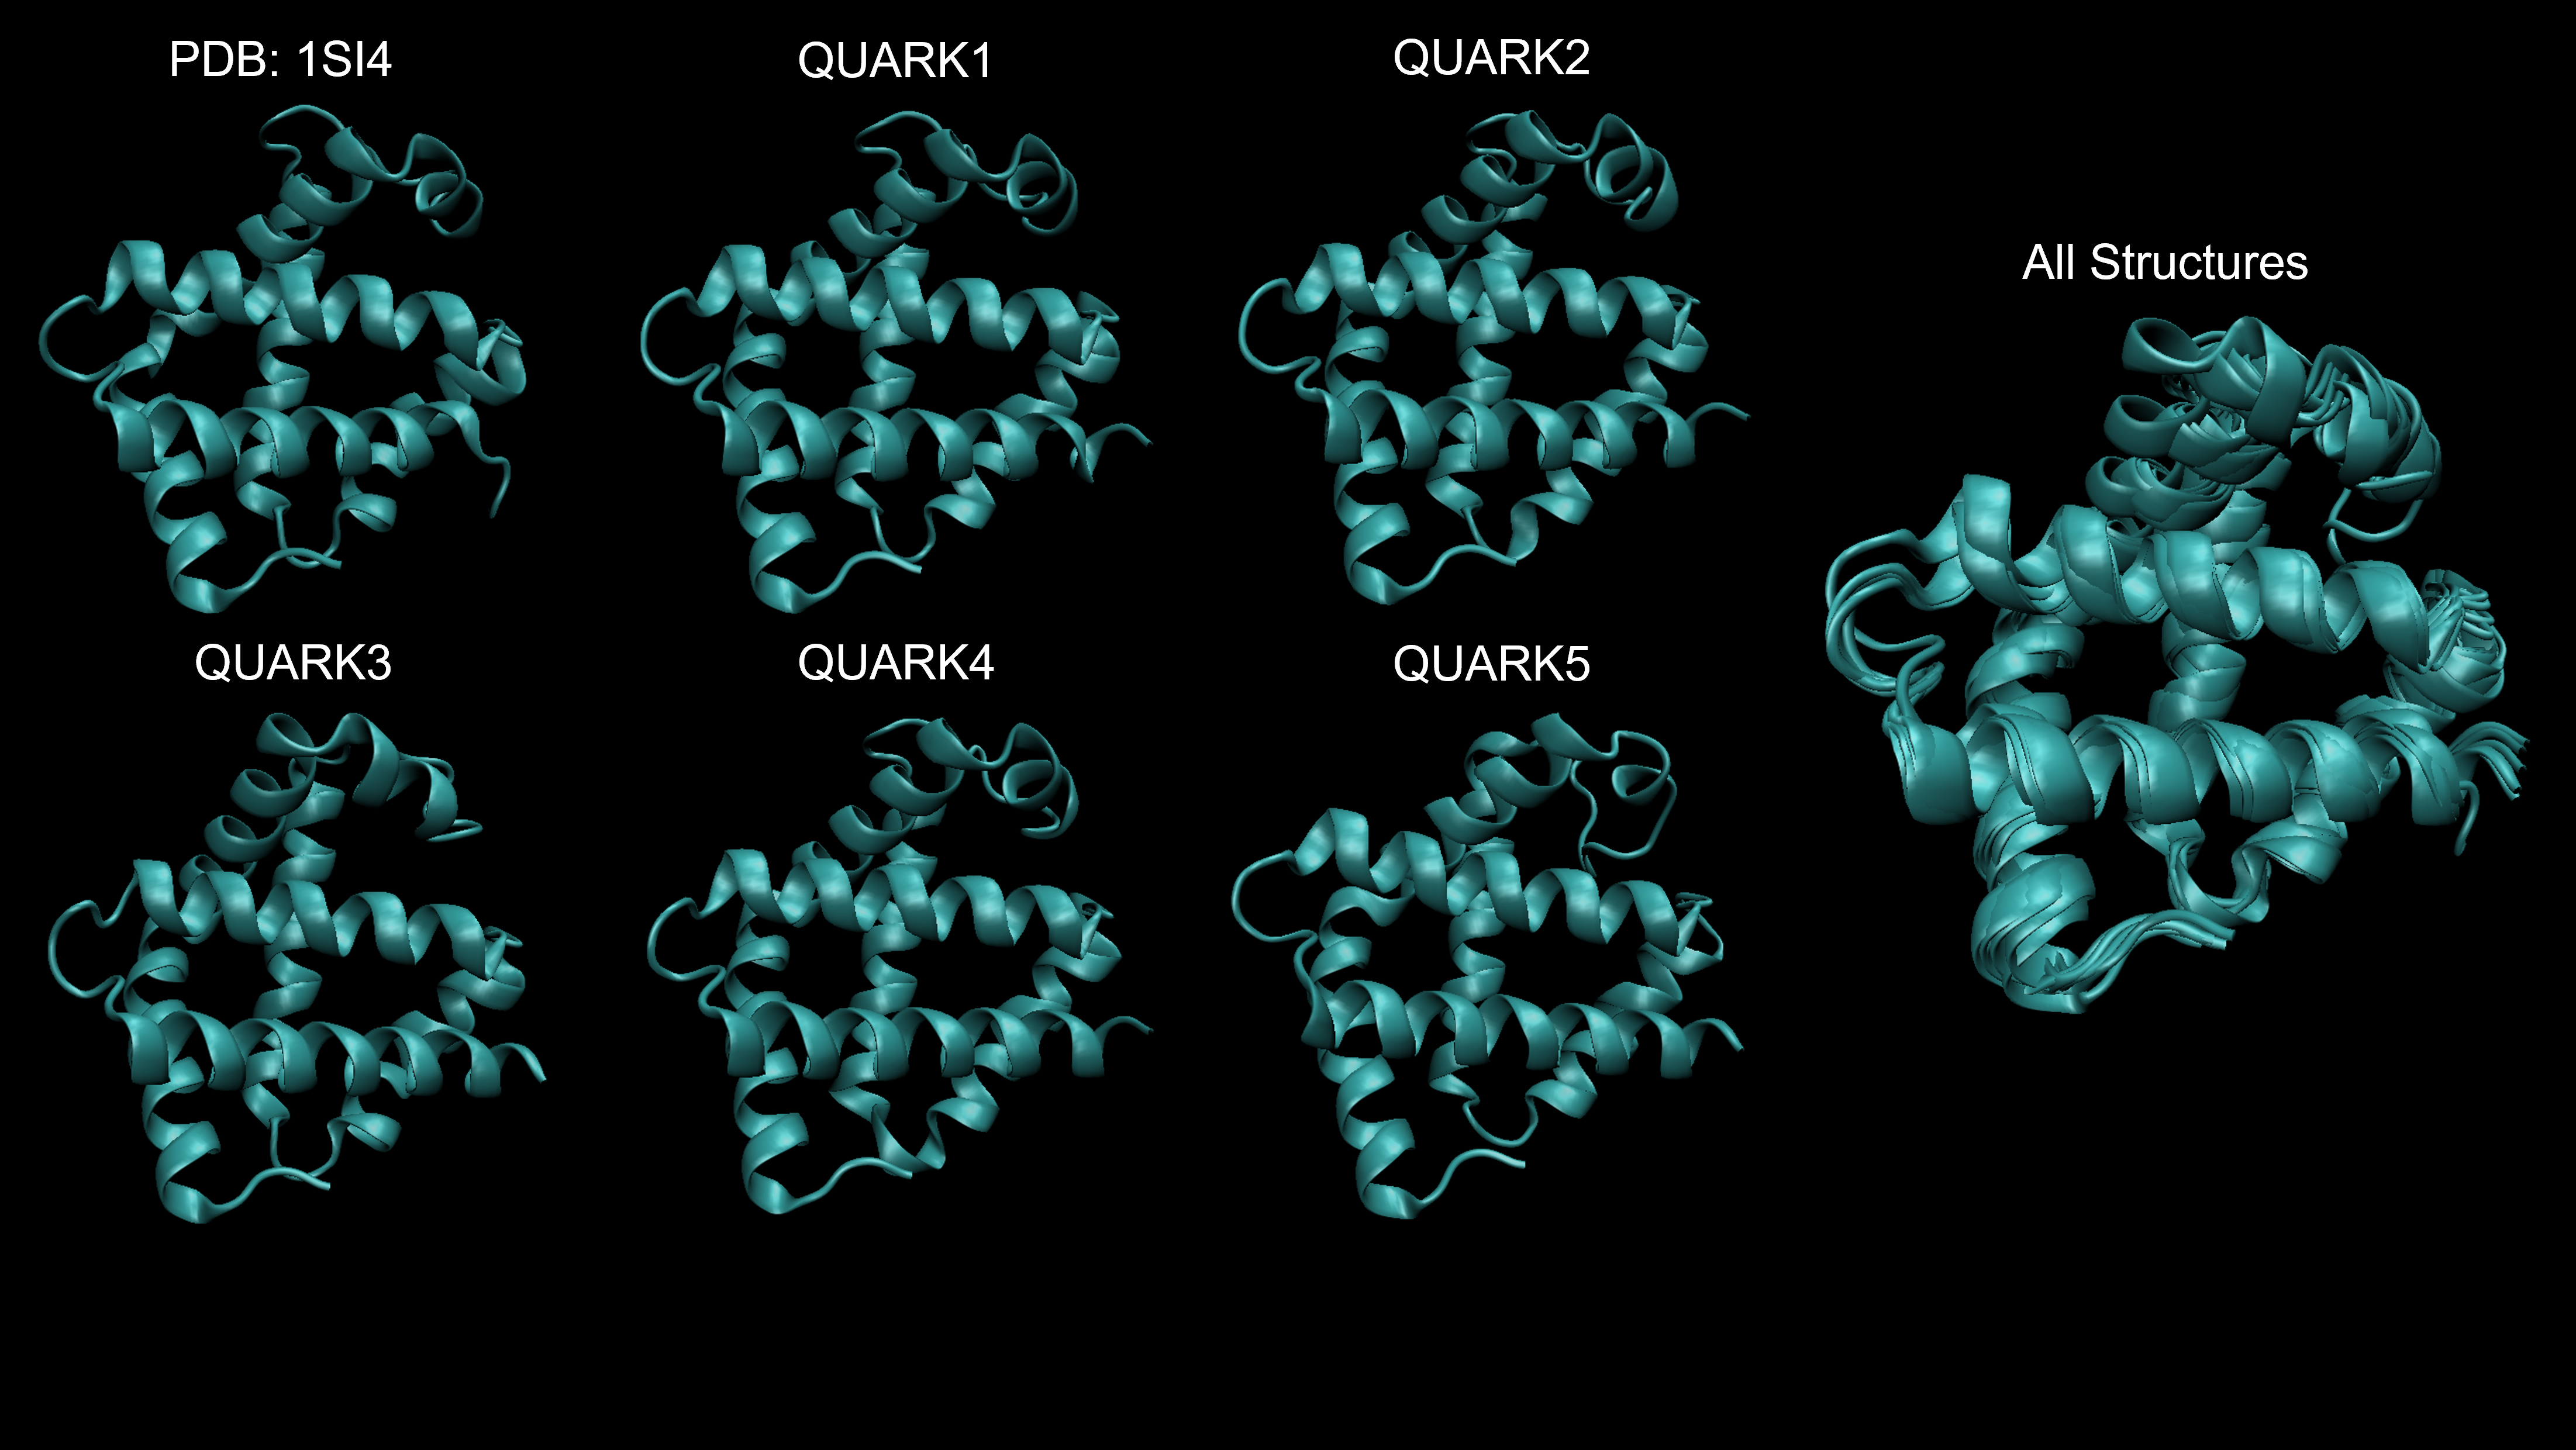
\includegraphics[width = 0.65\textwidth]{../images/ab_initio_results.png}
	\caption{The experimentally verified protein structure of human hemoglobin subunit alpha (top left) along with five models of this protein produced by QUARK from the protein's primary sequence, all of which are nearly indistinguishable from the verified structure with the naked eye.}
	\label{fig:ab_initio_results}
\end{figure}

%\begin{qbox}[%
%What known protein structure(s) would you first want to consult when studying the SARS-CoV-2 spike protein?
%]\end{qbox}

\FloatBarrier
\phantomsection

\section{Homology Modeling}
\label{sec:homology}
\phantomsection
\subsection{Using a known protein structure as a reference}

With every new protein structure that we identify experimentally, we gain a little more insight into nature's magic protein folding algorithm. In \textdef{homology modeling}{homology modeling}{an approach for protein structure prediction, also known as comparative modeling, in which we use the information contained in known structures to help us predict the structure of a protein with unknown structure} (also called \textdefnogloss{comparative modeling}), we use the information contained in known structures to help us predict the structure of a protein with unknown structure.

The structure of the SARS-CoV spike protein was determined in 2003. Assuming that the two proteins have similar structure, we will use SARS-CoV spike protein's known structure as a guide to help us predict the structure of the SARS-CoV-2 spike protein. In other words, we restrict the search space to those structures that are similar to the SARS-CoV spike protein structure.\\

\begin{qbox}[%
In the case of the SARS-CoV-2 spike protein, we already know that we want to use the SARS-CoV spike protein as a template. However, if we do not know which template to use before we begin, how could we find a candidate protein template?
]\end{qbox}

\phantomsection
\subsection{Finding a similar structure reduces the size of the search space}

Once we have found a protein with potentially similar structure to our protein of interest, we need to use this known structure to predict the structure of our protein. One way of doing so is to include a ``similarity term'' in the energy function that subtracts a structure's similarity to the template structure from the structure's total energy. That is, the more similar that a candidate structure is to the template, the more negative the contribution of this similarity term. To continue our search space analogy, the template protein ``pulls down'' the energy values of nearby structures like a gravity well.

Another way to perform homology modeling is to account for variance in similarity across different regions of the two proteins. The SARS-CoV and SARS-CoV-2 genomes are 96\% similar, but their spike proteins are only 76\% similar. In general, when we examine genomes from related species, we see \textdefnogloss{conserved regions} where the species are very similar and \textdefnogloss{variable regions} where the species are more different than the average.

The phenomenon of conserved and variable regions also occurs within individual genes. \autoref{fig:spike_protein_similarity} shows that within a spike protein subunit, the S2 domain is 90\% similar between the two viruses, whereas the S1 domain is only 64\% similar. Furthermore, the S1 domain divides into two subunits of differing similarity.\\

\begin{figure}[h]
	\centering
	\mySfFamily
	\includegraphics[width = 0.85\textwidth]{../images/spike_protein_similarity.png}\\
	\caption{Variable and conserved regions in the SARS-CoV and SARS-CoV-2 spike proteins. The S1 domain tends to be more variable, whereas the S2 domain is more conserved. In this figure, ``NTD'' stands for ``N-terminal domain'' and ``RBD'' stands for ``receptor binding domain'', two subunits of the S1 domain.}
	\label{fig:spike_protein_similarity}
\end{figure}

Some homology modeling algorithms account for variable and conserved regions by assuming that very conserved regions in the two genes correspond to essentially identical structures in the proteins. That is, the structure of our protein of interest in these regions will be the same as those of the template protein. We can then use a \textdefnogloss{fragment library}, a catalog of known substructures from many proteins, to fill in the structure of non-conserved regions based on structures of fragments whose sequence is similar to these regions. This approach is called \textdef{fragment assembly}{fragment assembly}{the process of using a library of known substructures from many proteins to fill in the structure of non-conserved regions when predicting a protein's structure}.

We will model the SARS-CoV-2 spike protein using homology modeling software from three publicly available fragment assembly servers (SWISS-MODEL, Robetta, and GalaxyWEB). If the results are similar, then we have faith in the \textit{robustness} of our predictions when using different approaches. Furthermore, comparing the results of multiple different approaches may give us more insights into structure prediction. \autoref{fig:homology_modeling_results_table} contains links to the results of running this software.\tutorial[coronavirus/tutorial_homology]

\begin{figure}[h]
	\centering
	\tabcolsep = 1 em
	\mySfFamily
	\begin{tabular}{c c}
		\textbf{Structure Prediction Server} & \textbf{Results} \\
		SWISS-MODEL (spike protein) & \url{https://bit.ly/3gIR1RC} \\
		Robetta (Single-Chain spike protein) & \url{https://bit.ly/34XMmsd} \\
		GalaxyWEB & \url{https://bit.ly/34WsKES} \\
	\end{tabular}
	\caption{A table containing links to the prediction results of three homology modeling software resources. SWISS-MODEL was used to predict the structure of the SARS-CoV-2 spike protein. Robetta was used to predict the structure of a single chain of the spike protein. GalaxyWEB was used to predict the structure of the spike protein's receptor binding domain (RBD).}
	\label{fig:homology_modeling_results_table}
\end{figure}

\phantomsection
\subsection{Experiments determine the structure of the SARS-CoV-2 spike protein}

On February 25, 2020, two months after the publication of the SARS-CoV-2 genome, researchers published the result of a cryo-EM experiment for the SARS-CoV-2 spike protein, which became PDB entry \href{http://www.rcsb.org/structure/6vxx}{6vxx}.\\

\begin{note}[%
	If you would like to explore the structure of the SARS-CoV-2 spike protein, check out the 3-D protein viewer at \url{https://www.rcsb.org/3d-view/6vxx}.
]\end{note}

We now turn to the problem of comparing our homology modeling results of the SARS-CoV-2 spike protein against the experimentally verified structure of SARS-CoV-2. How to compare two protein structures is a simple question, but it has a complicated answer, to which we will devote an entire section.\\

\FloatBarrier
\phantomsection

\section{Protein Structure Comparison}
\label{sec:accuracy}

\phantomsection
\subsection{Comparing two shapes with the Kabsch algorithm}

Comparing two protein structures is intrinsically similar to comparing two shapes, such as those in \autoref{fig:two_shapes}.\\

\begin{qbox}[%
	How similar are the two shapes in \autoref{fig:two_shapes}?
]\end{qbox}

\begin{figure}[h]
	\centering
	\mySfFamily
	\includegraphics[width = 0.7\textwidth]{../images/two_shapes.png}
	\caption{Two example shapes.}
	\label{fig:two_shapes}
\end{figure}

If you think you have a good handle on comparing the two shapes in \autoref{fig:two_shapes}, then it is because humans have very highly evolved eyes and brains. As we will see in \autoref{chapter:white_blood_cells}, training a computer to detect and differentiate objects is more difficult than you think!

We would like to develop a distance function $d(S, T)$ quantifying how different two shapes \textit{S} and \textit{T} are. If \textit{S} and \textit{T} are the same, then $d(S, T)$ should be equal to zero; the more different \textit{S} and \textit{T} become, the larger \textit{d} should become.

You may have noticed that the two shapes in \autoref{fig:two_shapes} are, in fact, identical. To demonstrate that this is true, we can first move the red shape to superimpose it over the blue shape, then flip the red shape, and finally rotate it so that its boundary coincides with the blue shape (\autoref{fig:shape_transformation}). In general, if a shape \textit{S} can be translated, flipped, and/or rotated to produce shape \textit{T}, then \textit{S} and \textit{T} are the same shape, and so $d(S, T)$ should be equal to zero. The question is what $d(S, T)$ should be if \textit{S} and \textit{T} are not the same shape.

\begin{figure}[p]
	\centering
	\tabcolsep = 1em
	\mySfFamily
	\begin{tabular}{c}
		\includegraphics[width = 0.6\textwidth]{../images/shape_transformation1.png}\\[2ex]
		\includegraphics[width = 0.25\textwidth]{../images/shape_transformation2.png} \\[2ex]
		\includegraphics[width = 0.25\textwidth]{../images/shape_transformation3.png}\\[2ex]
		\includegraphics[width = 0.25\textwidth]{../images/shape_transformation4.png} \\
	\end{tabular}
	\caption{(First panel) The two example shapes from \autoref{fig:two_shapes}. (Second panel) aligning the two shapes. (Third panel) Flipping the red shape across its vertical axis. (Fourth panel) Rotating the red shape reveals that it is identical to the blue shape.}
	\label{fig:shape_transformation}
\end{figure}

Our idea for defining $d(S, T)$, then, is first to translate, flip, and rotate \textit{S} so that it resembles \textit{T} ``as much as possible'' to give us a fair comparison. Once we have done so, we will devise a metric to quantify the difference between the two shapes that will represent $d(S, T)$.

We first translate \textit{S} to have the same \textdef{center of mass}{center of mass}{the point corresponding to a shape whose coordinates are the averages of respective coordinates of points on the shape} as \textit{T}. The center of mass of \textit{S} is found at the point $(x_{S}, y_{S})$ such that $x_{S}$ and $y_{S}$ are the respective averages of the \textit{x}-coordinates and \textit{y}-coordinates on the boundary of \textit{S}.

The center of mass of some shapes can be determined mathematically. But for irregular shapes, we will first sample \textvar{n} points from the boundary of \textvar{S} and then estimate $x_S$ and $y_S$ as the average of all the respective \textvar{x}- and \textvar{y}-coordinates from the sampled points.

After finding the centers of mass of the two shapes \textit{S} and \textit{T} that we wish to compare, we translate \textit{S} so that it has the same center of mass as \textit{T}. We then wish to find the rotation of \textit{S}, possibly along with a flip as well, that makes the shape resemble \textit{T} as much as possible.

Imagine that we have found the desired rotation; we are now ready to define $d(S, T)$ in the following way. We sample \textit{n} points along the boundary of each shape, converting \textit{S} and \textit{T} into \textdefnogloss{vectors} $\mathbf{s} = (s_{1}, \ldots, s_{n})$ and $\mathbf{t} = (t_{1}, \ldots, t_{n})$, where $s_{i}$ is the \textit{i}-th point on the boundary of \textit{S}. The \textdef{root mean square deviation (RMSD)}{root mean square deviation (RMSD)}{the square root of the average squared distance between corresponding points in two vectors} between the two shapes is the square root of the average squared distance between corresponding points in the vectors,

\begin{center}
$\text{RMSD}(\mathbf{s}, \mathbf{t}) = \sqrt{\dfrac{1}{n} \cdot \left(d(s_1, t_1)^2 + d(s_2, t_2)^2 + \cdots + d(s_n, t_n)^2\right)}$\,.
\end{center}

\noindent In this formula, $d(s_{i}, t_{i})$ is the distance between the points $s_{i}$ and $t_{i}$.\\

\begin{note}[%
	RMSD is a very commonly used approach across data science when measuring the differences between two vectors.
	]\end{note}

For an example two-dimensional RMSD calculation, consider \autoref{fig:rmsd_simple_shapes}, which shows two shapes with four points sampled from each. (Note: for simplicity, the shapes do not have the same center of mass.) The distances between corresponding points in this figure are equal to $\sqrt{2}$, 1, 4, and $\sqrt{2}$. As a result, we compute the RMSD as follows:
\begin{align*}
	\text{RMSD}(\mathbf{s}, \mathbf{t}) &= \sqrt{\dfrac{1}{4} \cdot (\sqrt{2}^2 + 1^2 + 2^2 + \sqrt{2}^2)} \\
	&= \sqrt{\dfrac{1}{4} \cdot 9}\\
	&= \sqrt{\dfrac{9}{4}}\\
	&= \dfrac{3}{2}
\end{align*}

\begin{figure}[h]
	\centering
	\mySfFamily
	\includegraphics[width = 0.7\textwidth]{../images/rmsd_simple_shapes.png}
	\caption{Two shapes with four points sampled from each.}
	\label{fig:rmsd_simple_shapes}
\end{figure}

\begin{qbox}[%
	Do you see any issues with using RMSD to compare two shapes?
]\end{qbox}

Even if we assume that two shapes have already been overlapped and rotated appropriately, we still should ensure that we sample enough points to give a good approximation of how different the shapes are. Consider a circle inscribed within a square (\autoref{fig:circle_square_undersampling}). If we happened to sample only the four points indicated, then we would sample the same points for each shape and conclude that the RMSD between these two shapes is equal to zero. Fortunately, this issue is easily resolved by making sure to sample enough points from the shape boundaries.\\

\begin{figure}[h]
	\centering
	\mySfFamily
	\includegraphics[width = 0.4\textwidth]{../images/circle_square_undersampling.png}
	\caption{A circle inscribed within a square. Sampling of the four points where the shapes intersect will give a flawed estimate of zero for the RMSD.}
	\label{fig:circle_square_undersampling}
\end{figure}

Throughout the above discussion, we have assumed that we already rotated (and possibly flipped) \textit{S} to be as ``similar'' to \textit{T} as possible. In practice, after superimposing \textit{S} and \textit{T} to have the same center of mass, we would like to find the flip and/or rotation of \textit{S} that \textit{minimizes} the RMSD between our vectorizations of \textit{S} and \textit{T} over all possible ways of flipping and rotating \textit{S}; fortunately, this flip and/or rotation can be found with an approach called the \textdef{Kabsch algorithm}{Kabsch algorithm}{an algorithm that identifies the best alignment of two shapes} that relies on some advanced linear algebra and is beyond the scope of this work. After applying the Kabsch algorithm to rotate and/or flip $S$, we set our desired distance $d(S, T)$ equal to the RMSD between the shapes' vectors of sampled points.

\phantomsection
\subsection{PDB format encodes a protein's structure}

The Kabsch algorithm offers a compelling way to determine the similarity of two protein structures. We can convert a protein containing \textit{n} amino acids into a vector of length \textit{n} by selecting a single representative point from each amino acid. We typically use the alpha carbon, the amino acid's centrally located carbon atom (recall the chemical structure of an amino acid from \autoref{fig:AminoAcid}).\\

\begin{figure}[h]
\centering
\mySfFamily
\scriptsize
\tabcolsep = 0.4em
\rowcolors{2}{gray!25}{white}
\begin{tabular}{c c c c c c c c c c}
\rowcolor{gray!50}
 & &  &  &  & & & \multicolumn{3}{c}{\textbf{Coordinates}}\\
\rowcolor{gray!50}
 & & \textbf{Index} & \textbf{Element} & \textbf{Amino acid} & \textbf{Chain} & \textbf{Position} & \textit{\textbf{x}} & \textit{\textbf{y}} & \textit{\textbf{z}}\\
\gray{2159} & ATOM & 1 & N & ALA& A & 27 & 171.646& 251.874& 224.877\\
\Green{2160} & \Green{ATOM} & \Green{2} & \Green{CA} & \Green{ALA}& \Green{A} & \Green{27} & \Green{172.298}& \Green{252.181} & \Green{223.613}\\
\gray{2161} & ATOM & 3 & C & ALA& A & 27 & 173.530& 251.298& 223.427\\
\gray{2162} & ATOM & 4 & O & ALA& A & 27 & 174.195& 250.943& 224.405\\
\gray{2163} & ATOM & 5 & CB & ALA& A & 27 & 172.700& 253.664& 223.554\\
\gray{2164} & ATOM & 6 & N & TYR& A & 28 & 173.816& 250.939& 222.166\\
\Green{2165} & \Green{ATOM} & \Green{7} & \Green{CA} & \Green{TYR} & \Green{A} & \Green{28} & \Green{174.968} & \Green{250.129} &\Green{221.763}\\
\gray{2166} & ATOM & 8 & C & TYR& A & 28 & 175.652& 250.729& 220.561\\
\gray{2167} & ATOM & 9 & O & TYR& A & 28 & 175.009& 251.379& 219.736\\
\gray{2168} & ATOM & 10 & CB & TYR& A & 28 & 174.546& 248.703& 221.426\\
\gray{2169} & ATOM & 11 & CG & TYR& A & 28 & 174.049& 247.932& 222.586\\
\gray{2170} & ATOM & 12 & CD1& TYR& A & 28 & 172.752& 248.072& 223.009\\
\gray{2171} & ATOM & 13 & CD2& TYR& A & 28 & 174.897& 247.067& 223.225\\
\gray{2172} & ATOM & 14 & CE1& TYR& A & 28 & 172.304& 247.348& 224.080\\
\gray{2173} & ATOM & 15 & CE2& TYR& A & 28 & 174.455& 246.338& 224.291\\
\gray{2174} & ATOM & 16 & CZ & TYR& A & 28 & 173.161& 246.477& 224.723\\
\gray{2175} & ATOM & 17 & OH & TYR& A & 28 & 172.710& 245.746& 225.795
\end{tabular}
\caption{Lines \text{2,159} to \text{2,175} of the \texttt{.pdb} file for the experimentally verified SARS-CoV-2 spike protein structure, PDB entry \href{http://www.rcsb.org/structure/6VXX}{6vxx}. These 17 lines contain information on the atoms taken from two amino acids, alanine and tyrosine. The rows corresponding to these amino acids' alpha carbons are shown in green and appear as ``CA'' under the ``Element'' column.  We have labeled the columns to make it clear what each column corresponds to: ``Index'' refers to the number of the amino acid; ``Element'' identifies the chemical element to which this atom corresponds; ``Chain'' indicates which chain the atom is found on; ``Position'' identifies the position in the protein of the amino acid from which the atom is taken; ``Coordinates'' indicates the \textvar{x}, \textvar{y}, and \textvar{z} coordinates of the atom's location (in angstroms).}
\label{fig:simplifiedPDB}
\end{figure}

Whether a protein structure is experimentally validated or predicted by an algorithm, the structure is often represented in a unified file format used by the PDB called \texttt{.pdb} format (\autoref{fig:simplifiedPDB}). In this format, each atom in the protein is labeled according to several different characteristics, including: the element from which the atom derives; the amino acid in which the atom is contained; the chain on which this amino acid is found; the position of the amino acid within this chain; and the 3D coordinates $(x, y, z)$ of the atom in angstroms ($10^{-10}$ meters).\\

\begin{note}[%
	\autoref{fig:simplifiedPDB} shows just part of the information needed to fully represent a protein structure. For example, a \texttt{.pdb} file will also contain information about the disulfide bonds between amino acids. For more information, consult the \href{http://www.wwpdb.org/documentation/file-format}{official PDB documentation}.
	]\end{note}

\phantomsection
\subsection{The Kabsch algorithm can be fooled}

Although the Kabsch algorithm is powerful, we should be careful when using it. Consider \autoref{fig:RMSD_weakness_mutation}, which shows two toy protein structures; the orange structure (\textit{S}) is identical to the blue structure (\textit{T}) except for a change in a single bond angle between the third and fourth amino acids. And yet this tiny change in the protein's structure causes a significant increase in $d(s_{i}, t_{i})$ for every \textit{i} greater than 3, which inflates the RMSD.

\begin{figure}[p]
	\centering
	\mySfFamily
	\includegraphics[width = 0.85\textwidth]{../images/RMSD_weakness_mutation.png}
	\caption{(Top) Two hypothetical protein structures that differ in only a single bond angle between the third and fourth amino acids, shown in red. Each circle represents an alpha carbon. (Bottom left) Superimposing the first three amino acids shows how much the change in the bond angle throws off the computation of RMSD by increasing the distances between corresponding alpha carbons. (Bottom right) The Kabsch algorithm would align the centers of gravity of the two structures in order to minimize RMSD between corresponding alpha carbons. This alignment belies the similarity in the structures and makes it difficult for the untrained observer to notice that the two proteins only differ in a single bond angle.}
	\label{fig:RMSD_weakness_mutation}
\end{figure}

Another way in which the Kabsch algorithm can be tricked is in the case of an appended substructure that throws off the ordering of the amino acids. \autoref{fig:RMSD_weakness_loop} shows a toy example of a structure into which we incorporate a loop, thus throwing off the natural order of comparing amino acids. (The same effect is caused if one or more amino acids are deleted from one of the two proteins.)

\begin{figure}[t]
	\centering
	\mySfFamily
	\includegraphics[width = 0.7\textwidth]{../images/RMSD_weakness_loop.png}
	\caption{Two toy protein structures, one of which (bottom) includes a loop of three amino acids. After the loop, each amino acid in the orange structure will be compared against an amino acid that occurs farther long in the blue structure, thus increasing $\textvar{d}(\textvar{s}_{\textvar{i}}, \textvar{t}_{\textvar{i}})$ for each such amino acid and inflating RMSD.}
	\label{fig:RMSD_weakness_loop}
\end{figure}

To address this second issue, biologists will often align the sequences of two proteins first, discarding any positions that do not align well when it comes time to perform the RMSD calculation. We will soon see an example of a protein sequence alignment when comparing the coronavirus spike proteins.

In short, if the RMSD of two proteins is \textit{large}, then we should be wary of concluding that the proteins are very different, and we may need to combine RMSD with other methods of structure comparison. But if the RMSD is \textit{small} (e.g., just a few angstroms), then we can have confidence that the proteins are indeed similar.

We are now ready to apply the Kabsch algorithm to compare the structures that we predicted for human hemoglobin subunit alpha and the SARS-CoV-2 spike protein against their experimentally validated structures. \tutorial[coronavirus/tutorial_rmsd]

\FloatBarrier
\phantomsection
\subsection{Assessing the accuracy of our structure prediction models}

Earlier in this chapter, we used publicly available protein structure prediction servers to predict the structure of human hemoglobin subunit alpha (using \textit{ab initio} modeling) and the SARS-CoV-2 spike protein (using homology modeling). We will now see how well our models performed by showing the values of RMSD produced by the Kabsch algorithm when comparing each of these models against the validated structures.

\autoref{fig:quark_rmsd_table} shows the RMSD between each of the five predicted structures returned by QUARK and the validated structure of human hemoglobin subunit alpha. We are tempted to conclude that our \textit{ab initio} prediction was a success. However, because human hemoglobin subunit alpha is so short (141 amino acids), researchers would consider this RMSD score to be high.\fudgespace

\begin{figure}[h]
	\centering
	\tabcolsep = 1 em
	\mySfFamily
	\begin{tabular}{c c}
		\textbf{QUARK Models} & \textbf{RMSD} \\
		QUARK 1 & 1.58\phantom{xx} \\
		QUARK 2 & 2.0988\\
		QUARK 3 & 3.11\phantom{xx} \\
		QUARK 4 & 1.9343\\
		QUARK 5 & 2.6495
	\end{tabular}
	\caption{The RMSD of five models of human hemoglobin subunit alpha predicted by QUARK compared against the protein's validated structure (PDB entry: \href{https://www.rcsb.org/structure/1si4}{1si4}).}
	\label{fig:quark_rmsd_table}
\end{figure}


\FloatBarrier
\phantomsection
\subsection{Homology models of the SARS-CoV-2 spike protein}

We also used GalaxyWeb to predict the structure of the SARS-CoV-2 spike protein's RBD, Robetta to predict the structure of a single chain, and SWISS-MODEL to predict the structure of the entire protein. \autoref{fig:sars-cov-2_rmsd_table} compiles the RMSD of structures predicted by this homology modeling software against experimental results.\\

\begin{figure}[h]
	\centering
	\tabcolsep = 1 em
	\mySfFamily
	\begin{tabular}{c c}
		\textbf{Predicted Structure} & \textbf{RMSD} \\
		GalaxyWEB 1 & \phantom{x}0.1775 \\
		GalaxyWEB 2 & \phantom{x}0.1459 \\
		GalaxyWEB 3 & \phantom{x}0.1526 \\
		GalaxyWEB 4 & \phantom{x}0.1434 \\
		GalaxyWEB 5 & \phantom{x}0.1202 \\
		Robetta 1 & \phantom{x}3.1189 \\
		Robetta 2 & \phantom{x}3.7568 \\
		Robetta 3 & \phantom{x}2.9972 \\
		Robetta 4 & \phantom{x}2.5852 \\
		Robetta 5 & 12.0975 \\
		SWISS-Model 1 & \phantom{x}5.8518 \\
		SWISS-Model 2 & 11.3432 \\
		SWISS-Model 3 & 11.3432 \\
	\end{tabular}
	\caption{A table containing the RMSD of SARS-CoV-2 spike protein structures predicted by software against the known structure. GalaxyWEB's results are compared against the RBD (PDB entry: \href{https://www.rcsb.org/structure/6lzg}{6lzg}); Robetta's results are compared against a single chain, and SWISS-Model's are compared against the entire protein (PDB entry: \href{https://www.rcsb.org/structure/6vxx}{6vxx}).}
	\label{fig:sars-cov-2_rmsd_table}
\end{figure}

The GalaxyWEB models have an excellent RMSD score and can be considered very accurate. Note that their RMSD is more than an order of magnitude lower than the RMSD computed for our \textit{ab initio} predictions of hemoglobin subunit alpha, despite the fact that the RBD is longer (229 amino acids). As for the other two software resources, although the RMSD values are higher than those of GalaxyWEB, keep in mind that a single chain of the spike protein is 1,281 amino acids long, and so the sensitivity of RMSD to slight changes should give us confidence that our models are on the right track.\\

\begin{qbox}[%
	Which do you think performed more accurately on our predictions: SWISS-MODEL or Robetta?
]\end{qbox}

\phantomsection
\subsection{Distributing the work of protein structure prediction around the world}

Two leading structure prediction projects, \href{https://boinc.bakerlab.org}{Rosetta@home} and \href{https://foldingathome.org}{Folding@home}, encourage volunteers to download their software and contribute to a gigantic \textit{distributed} effort to predict protein shape. Even with a modest laptop, a user can donate some of their computer's idle resources to contribute to the problem of protein structure prediction. While some researchers were working to elucidate the structure of the SARS-CoV-2 spike protein experimentally, thousands of users were devoting their computers to the cause of predicting the protein's structure computationally.

The RMSD values for the models predicted by Rosetta@Home are shown in \autoref{fig:ssgcid_rmsd_table}. As we might expect due to having access to thousands of users' computers, these models outperform our own from \autoref{fig:sars-cov-2_rmsd_table}. Yet a typical threshold for whether a predicted structure is accurate is if its RMSD compared to a validated structure is smaller than 2.0 angstroms, a test that the models in \autoref{fig:ssgcid_rmsd_table} do not pass.

\begin{figure}[h]
	\centering
	\tabcolsep = 1 em
	\mySfFamily
	\begin{tabular}{c c c}
		\textbf{Rosetta@Home Models} & \textbf{RMSD (Single Chain)} & \textbf{RMSD (Full Protein)}\\
		Model 1  & 2.7843 & 3.505\phantom{x}  \\
		Model 2  & 2.107\phantom{x} & 2.3274 \\
		Model 3  & 1.866\phantom{x} & 2.12\phantom{xx} \\
		Model 4  & 2.047\phantom{x} & 2.0854 \\
		Model 5  & 4.6443 & 4.9636
	\end{tabular}
	\caption{A table containing the the calculated RMSD of the Rosetta@Home models of SARS-CoV-2 spike protein, full protein and single chain, compared to the validated structure (PDB entry: \href{https://www.rcsb.org/structure/6vxx}{6vxx}).}
	\label{fig:ssgcid_rmsd_table}
\end{figure}

The inability of even powerful models to obtain an accurate predicted structure may make it seem that protein structure prediction is a lost cause. Perhaps biochemists should head back to expensive experimental validations and ignore the musings of computational scientists. In the next section, which serves as the midpoint of this chapter, we will find hope.\\

\phantomsection

\section{Intermezzo: Did AlphaFold Solve the Protein Structure Prediction Problem?}
\label{sec:intermezzo}
\phantomsection

Protein structure prediction is an old problem. In 1967, the Soviets founded an entire research institute dedicated to solving ``the protein problem''; this institute still lives on today. Despite the difficulty of protein structure prediction, gradual algorithmic improvements and increasing computational resources have led biologists around the world to wish for the day when they could consider protein structure prediction to be solved.

That day has come. Kind of.

Every two years since 1994, a global contest called \textdefnogloss{Critical Assessment of protein Structure Prediction (CASP)} has allowed modelers to test their protein structure prediction algorithms against each other. The contest organizers compile a (secret) collection of experimentally verified protein structures and then run all submitted algorithms against these proteins.

In 2020, the 14th iteration of this contest (CASP14) was won in a landslide. The second version of \href{https://bit.ly/3sKl6pH}{\textdefnogloss{AlphaFold}}, a DeepMind project, vastly outperformed the world's foremost structure prediction approaches. The algorithm powering AlphaFold is an extremely involved method based on deep learning, a topic that we will touch upon in \autoref{chapter:white_blood_cells}.

Instead of using RMSD, CASP scores a predicted structure against a known structure using the \textdefnogloss{global distance test (GDT)}. We first ask, ``How many corresponding alpha carbons are close to each other in the two structures?'' To answer this question, we take the percentage of corresponding alpha carbon positions having distance apart that is at most equal to some threshold \textit{t}. The GDT score averages the percentages obtained when \textit{t} is equal to each of 1, 2, 4, and 8 angstroms. A GDT score of 90\% is considered good, and a score of GDT 95\% is considered excellent (i.e., comparable to minor errors resulting from experimentation).

We will show a few plots to illustrate the decisiveness of AlphaFold's CASP14 victory. In \autoref{fig:AlphaFold2_BAKER_Zhang} (top), we compare the GDT scores of AlphaFold against the second-place algorithm (a product of David Baker's laboratory, which developed the Robetta and Rosetta@Home software that we encountered in this chapter). We can appreciate the size of this margin of victory if we compare it against the difference between the second and third place competitors (\autoref{fig:AlphaFold2_BAKER_Zhang} (bottom)).\\

\begin{figure}[h]
	\centering
	\mySfFamily
	\includegraphics[width = 0.85\textwidth]{../images/AlphaFold2_BAKER.png}\\[4ex]
	\includegraphics[width = 0.85\textwidth]{../images/BAKER_Zhang.png}
	\caption{(Top) A plot of GDT scores for the AlphaFold2 (blue) and Baker lab (orange) submissions over all proteins in the CASP14 contest. AlphaFold2 finished first in CASP14, and Baker lab finished second. (Bottom) A plot of GDT scores for the Baker lab (blue) and Zhang lab (orange) submissions for all proteins in the CASP14 contest. Zhang lab finished third in CASP14.}
	\label{fig:AlphaFold2_BAKER_Zhang}
\end{figure}

For each protein in the CASP14 contest, we can also compute each algorithm's \textdefnogloss{z-score}, defined as the number of standard deviations that the algorithm's GDT score falls from the mean GDT score over all competitors. For example, a z-score of 1.4 would imply that the approach performed 1.4 standard deviations above the mean, and a z-score of $-0.9$ would imply that the approach performed 0.9 standard deviations below the mean.

By summing all of an algorithm's positive z-scores, we obtain a reasonable metric for the relative quality of an algorithm compared to its competitors. If this sum of z-scores is large, then the algorithm racked up lots of positive z-scores, meaning that it is performing significantly above average on the prediction of some proteins. \autoref{fig:CASP14_overall_results} shows the sum of z-scores for all CASP14 participants and reiterates the margin of AlphaFold's victory, since its sum of z-scores was twice that of the second place algorithm.

\begin{figure}[h]
	\centering
	\mySfFamily
	\includegraphics[width = 0.85\textwidth]{../images/CASP14_overall_results.png}
	\caption{A bar chart plotting the sum of z-scores for every entrant in the CASP14 contest. AlphaFold2 is shown on the far left; its sum of z-scores is over double that of the second-place submission.}
	\label{fig:CASP14_overall_results}
\end{figure}

AlphaFold's CASP14 triumph led some scientists --- and media outlets --- to declare that protein structure prediction had finally been solved. Yet some critics remained skeptical.

Although AlphaFold obtained an impressive median RMSD of 1.6 angstroms for its predicted proteins, about a third of these predictions have an RMSD over 2.0 angstroms, which we mentioned earlier is often used as a threshold for whether a predicted structure is reliable. We will not know in advance whether AlphaFold's predicted structure is outside of this range unless we experimentally validate the protein's structure.

Furthermore, some experts have claimed that to be completely trustworthy for a sensitive application like designing drugs to target proteins implicated in diseases, the RMSD of predicted protein structures would need to be nearly an order of magnitude lower, i.e., closer to 0.2 angstroms.

Finally, the AlphaFold algorithm is ``trained'' using a database of known protein structures, which makes it more likely to succeed if a protein is similar to a known structure. But the proteins with structures that are \textit{dissimilar} to any known structure are the ones possessing some of the greatest scientific interest.

Pronouncing protein structure prediction to be solved may be hasty, but we will likely never again see such a clear improvement to the state of the art for structure prediction. AlphaFold represents, perhaps, the final great innovation for a research problem that has puzzled biologists for over half a century.

Thus ends our discussion of protein structure prediction, but we still have much more to say. In particular, when comparing two protein structures, we have relied only upon the RMSD between the vectorizations of these two structures after applying the Kabsch algorithm. But using a single statistic to represent the differences between two protein structures belies what those differences might be. Furthermore, proteins are not static objects; they bend and shape in their environment as they perform their tasks. We will therefore now transition into a second part of our treatment of protein analysis, in which we investigate additional methods used to compare proteins and apply these techniques to the validated structures of the SARS-CoV and SARS-CoV-2 spike proteins.\\

\FloatBarrier
\phantomsection

\section{Finding Local Differences in Protein Structures with Qres}
\label{sec:multiseq}
\phantomsection

\FloatBarrier
\phantomsection
\subsection{Focusing on a variable region of interest in the spike protein}

The spike protein is much more variable than other regions of the coronavirus genome, and as we showed in \autoref{fig:spike_protein_similarity}, the protein has some regions of greater variability.  One such region is the RBD, which includes the \textdefnogloss{receptor binding motif (RBM)}, a subregion whose amino acid product mediates contact with the human ACE2 enzyme and is part of the RBD, whose structure we predicted using GalaxyWEB.

The fact that the region binding to the target human enzyme has mutated so much makes it a fascinating region of study. Do the mutations that SARS-CoV-2 has accumulated somehow make it easier for the virus to infect human cells?

\autoref{fig:RBM_alignment} shows an alignment of the 70 amino acid long RBM region from SARS-CoV and SARS-CoV-2. We know from our work in structure prediction that just because the sequence of a protein has been greatly mutated does not mean that the structure of that protein has changed much. Therefore, we will start a \textit{structural} comparison of the SARS-CoV and SARS-CoV-2 spike proteins.

\begin{figure}[h]
	\centering
	\mySfFamily
	\begin{sequence}[0.58]%
	\Green{NTRNIDATSTGNYNYKYR}YL\Green{R}HGK\Green{L}R\Green{PFERDIS}NVPFSPDGK\Green{PC}TP-PAL\Green{NCY}W\Green{PL}ND\Green{YGF}YT\Green{T}T\Green{G}I\Green{GYQPY}-\\
	\Green{NTRNIDATSTGNYNYKYR}LF\Green{R}KSN\Green{L}K\Green{PFERDIS}TEIYQAGST\Green{PC}NGVEGF\Green{NCY}F\Green{PL}QS\Green{YGF}QP\Green{T}N\Green{G}V\Green{GYQPY}-
	\end{sequence}
	\caption{An alignment of the RBM of the human SARS-CoV virus (first row) and the SARS-CoV-2 virus (second row). Amino acids that are highlighted in green represent matches between the two RBM sequences.}
	\label{fig:RBM_alignment}
\end{figure}

In addition to verifying the structure of the spike protein in both SARS-CoV and SARS-CoV-2, researchers also determined the structure of the RBD complexed with ACE2 in both SARS-CoV (PDB entry: \href{https://www.rcsb.org/structure/2ajf}{2ajf}) and SARS-CoV-2 (PDB entry: \href{https://www.rcsb.org/structure/6vw1}{6vw1}). Because we know the structures of the bound complexes, we can produce 3-D visualizations of the two different complexes and look for structural differences involving the RBM, rotating the structures around to examine potential differences. However, we should be wary of only trusting our eyes to guide us; how can a quantitative approach tell us where to look for structural differences between the two RBMs?\\

\begin{note}[%
	The experimentally verified SARS-CoV-2 structure is a \textit{chimeric} protein formed of the SARS-CoV RBD in which the RBM has the sequence from SARS-CoV-2. A chimeric RBD was used for complex technical reasons to ensure that the crystallization process during X-ray crystallography could be borrowed from that used for SARS-CoV.
	]\end{note}

\FloatBarrier
\phantomsection
\subsection{Contact maps visualize global structural differences}

Recall the following definition of RMSD for two protein structures \textvar{s} and \textvar{t}, in which each structure is represented by the positions of its \textvar{n} alpha carbons $(s_{1}, \cdots, s_{n})$ and $(t_{1}, \cdots, t_{n})$:

\begin{center}
$\text{RMSD}(s, t) = \sqrt{\dfrac{1}{n} \cdot (d(s_1, t_1)^2 + d(s_2, t_2)^2 + \cdots + d(s_n, t_n)^2)}$\,.
\end{center}

\noindent RMSD offers an excellent method for a \textit{global} comparison (i.e., a comparison across all structures), but we are interested in investigating the \textit{local} regions where the SARS-CoV and SARS-CoV-2 complexes differ.

If two similar protein structures differ in a few locations, then the corresponding alpha carbon distances $d(s_{i}, t_{i})$ will likely be higher at these locations. However, one of the weaknesses of RMSD that we pointed out earlier is that a change to a single bond angle at the \textvar{i}-th position may cause $d(s_{j}, t_{j})$ to be nonzero when $j > i$, even though the structure of the protein downstream of this bond angle has not changed. For example, recall \autoref{fig:RMSD_weakness_mutation} from our discussion of the Kabsch algorithm, in which we showed two toy protein structures that are identical except for a single bond angle. All the alpha carbon distances $d(s_{i}, t_{i})$ for \textvar{i} at least equal to 4 will be thrown off by this changed angle.

However, note in \autoref{fig:RMSD_weakness_mutation}  that when \textvar{i} and \textvar{j} are both at least equal to 4, the distance $d(s_{i}, s_{j})$ between the \textvar{i}-th and \textvar{j}-th alpha carbons in \textvar{S} will still be similar to the distance $d(t_{i}, t_{j})$ between the same alpha carbons in \textvar{T}. This observation leads us to a more robust approach for measuring differences in two protein structures, which compares \textvar{all} pairwise intraprotein distances $d(s_{i}, s_{j})$ in one protein structure against the corresponding distances $d(t_{i}, t_{j})$ in the other structure.

To help us visualize all these pairwise distances, we will introduce the \textdef{contact map}{contact map}{a binary matrix used to determine which pairs of alpha carbons in two proteins are close to each other} of a protein structure \textvar{s}, which is a binary matrix indicating whether two alpha carbons are near each other in \textvar{s}. After setting a threshold distance, we set $M(i, j) = 1$ if the distance $d(s_{i}, s_{j})$ is less than the threshold, and we set $M(i, j) = 0$ if $d(s_{i}, s_{j})$ is greater than or equal to the threshold.

\autoref{fig:contact_map} shows the contact maps for the SARS-CoV-2 and SARS-CoV spike proteins (both full proteins and single chains) with a threshold distance of twenty angstroms. In this map, we color contact map values black if they are equal to 1 (close amino acid pairs) and white if they are equal to 0 (distant amino acid pairs).\\

\begin{note}[%
	Interested in learning how to make contact maps? We will do so in a tutorial soon.
	]\end{note}

We observe two facts about the contact maps in \autoref{fig:contact_map}. First, many black values cluster around the main diagonal of the matrix, since amino acids that are nearby in the protein sequence will remain near each other in the 3-D structure. Second, the contact maps for the two proteins are very similar, reinforcing that the two proteins have similar structures. In general, contact map regions showing differences for two proteins provide regions for further investigation when comparing proteins structurally.\\

\begin{figure}[h]
	\centering
	\mySfFamily
	\includegraphics[width = 0.85\textwidth]{../images/Contact.png}
	\caption{The contact maps of the SARS-CoV-2 spike protein (top left), SARS-CoV spike protein (top right), single chain of the SARS-CoV-2 spike protein (bottom left), and single chain of the SARS-CoV spike protein (bottom right). If the distance between the \textvar{i}-th and \textvar{j}-th amino acids in a protein structure is 20 angstroms or less, then the (\textvar{i}, \textvar{j})-th cell of the figure is colored black. The SARS-CoV-2 and SARS spike proteins have very similar contact maps, indicating similar global structures.}
	\label{fig:contact_map}
\end{figure}

\begin{qbox}[%
	How do you think a contact map will change as we increase or decrease the threshold distance used to produce that map?
	]\end{qbox}

\FloatBarrier
\phantomsection
\subsection{Qres measures local structural differences}

We obtain some insight into how two proteins differ structurally at the \textvar{i}-th amino acid if we look at the values in the \textvar{i}-th row of the proteins' contact maps; that is, if we compare all the $d(s_{i}, s_{j})$ values to all the $d(t_{i}, t_{j})$ values. In practice, researchers combine all this information into a single metric called \textdefnogloss{Q per residue (Qres)} measuring the similarity of two structures at the \textvar{i}-th amino acid. The formal definition of Qres for two structures \textvar{s} and \textvar{t} having \textvar{N} amino acids is

\begin{center}
$Q_{\text{res}}^{(i)} = \dfrac{1}{N-k} \displaystyle \sum^{N}_{j\neq i-1,i,i+1} \exp\left[-\dfrac{[d(s_i,s_j)-d(t_i,t_j)]^2}{2\sigma^2_{i,j}}\right]$\,.
\end{center}

\noindent In this equation, $\exp(x)$ denotes $e^{x}$; \textvar{k} is equal to 2 at either the start or the end of the protein (i.e., \textvar{i} is equal to 1 or \textvar{N}), and \textvar{k} is equal to 3 otherwise; and the variance term $\sigma_{ij}^2$ is equal to $\left\lvert{i-j}\right\rvert ^{0.15}$, which corresponds to the sequence separation between the \textvar{i}-th and \textvar{j}-th alpha carbons.\\

\begin{note}[%
	The above definition of Qres assumes that the two proteins have the same length or have been pre-processed by removing amino acids that only occur in one protein. Generalizations of Qres for proteins of non-equal length exist that first align proteins and retain only those amino acids for structural comparison that are shared by the two proteins.
	]\end{note}

If two proteins are very similar at the \textvar{i}-th alpha carbon, then for every \textvar{j}, the difference $d(s_{i}, s_{j}) - d(t_{i}, t_{j})$ will be close to zero, meaning that each term inside the summation in the Qres equation will be close to 1. The sum will be equal to approximately $N - k$, and so Qres will be close to 1. As two proteins become more different at the \textvar{i}-th alpha carbon, then the term inside the summation will head toward zero, and so will the value of Qres.

Qres is therefore a metric of similarity ranging between 0 and 1. Low scores indicate low similarity between two proteins at the \textvar{i}-th position, and higher scores indicate high similarity at this position. We are now ready to apply Qres to the SARS-CoV and SARS-CoV-2 spike proteins and visualize the individual locations where the two proteins' RBD regions differ.\tutorial[coronavirus/tutorial_multiseq]

\FloatBarrier
\phantomsection
\subsection{Local comparison of spike proteins leads us to a region of interest}

By computing Qres at every position of the two coronavirus RBD regions, we can form a \textdefnogloss{structural alignment} of the two regions (\autoref{fig:QresResult}). Blue columns correspond to amino acids with high Qres (meaning high structural similarity), and red columns correspond to amino acids with low Qres (meaning low structural similarity). If we zoom in on the region around position 150 of the alignment, then we find a 13-column region of the alignment within the RBD region for which Qres values are significantly lower than they are elsewhere. This region corresponds to positions 476 to 485 in the SARS-CoV-2 spike protein, which is part of the RBM.\\

\begin{figure}[h]
	\centering
	\mySfFamily
		\includegraphics[width = 0.85\textwidth]{../images/QresResult.png} \\
	\caption{A snapshot of the sequence alignment between the SARS-CoV RBD (first row) and the SARS-CoV-2 chimeric RBD (second row). Columns are colored along a spectrum from blue (high Qres) to red (low Qres), with positions that correspond to an inserted or deleted amino acid colored red. The region with low Qres corresponds to amino acids at positions 476 to 485 in the SARS-CoV-2 spike protein.}
	\label{fig:QresResult}
\end{figure}

\autoref{fig:QresVMD} shows a 3-D visualization of the ACE2 enzyme (green) bound with the superimposed structures of both the SARS and SARS-CoV-2 RBD. The same color-coding of columns of the multiple alignment in \autoref{fig:QresResult} (top) is used to color positions in the superimposed RBDs; we have outlined the low-Qres region of the RBM alignment that we highlighted in \autoref{fig:QresResult} (bottom).\\

\begin{figure}[h]
	\centering
	\mySfFamily
	\includegraphics[width = 0.6\textwidth]{../images/QresVMD.png}
	\caption{A visualization showing the superimposed structures of the SARS-CoV-2 chimeric RBD  and SARS-CoV RBD, with individual amino acids colored blue or red depending on whether Qres is high or low, respectively.  The ACE2 enzyme is shown in green. The boxed region corresponds to the part of the RBM having a potential structural difference. Because this region is adjacent to ACE2, the structural difference will likely affect ACE2 interactions.}
	\label{fig:QresVMD}
\end{figure}

\begin{note}[%
	Although the rest of the proteins are similar, there are other parts of the RBD at the top of the protein that show dissimilarities in the two proteins, which may be attributable to an experimental artifact. The authors of the work in which the comparison was published pointed out that the highlighted region is unlikely to be an artifact of the experimentation because it is ``buried at the RBD–ACE2 interface and did not affect crystallization''.
	]\end{note}

Finding a region in the RBM where the structures of the SARS-CoV and SARS-CoV-2 spike proteins differ presents an exciting development. We will next explore this region of the protein structure along with two others identified by researchers to determine whether the mutations acquired by SARS-CoV-2 may have influenced the binding affinity of the virus spike protein with the human ACE2 enzyme. Structural differences are challenging to show with a 2-D image, and we encourage you to generate the 3-D representation of the protein in a tutorial.\tutorial[coronavirus/tutorial_visualization]\\

\FloatBarrier
\phantomsection
\section{Analysis of Structural Protein Differences in the Spike Protein}
\label{sec:structural_differences}

\phantomsection
\subsection{Site 1: loop in the ACE2-binding ridge}

The first location that we will consider is our region of interest identified in the previous section, which is found on a loop in a region called the ACE2 binding ridge. This region is highlighted in \autoref{fig:Ridge} for SARS-CoV-2 (left) and SARS-CoV (right).

\begin{figure}[h]
	\centering
	\mySfFamily
	\begin{tabular}{c c}
	\includegraphics[width = 0.4\textwidth]{../images/Ridge_SARS-2.png} & \includegraphics[width = 0.4\textwidth]{../images/Ridge_SARS.png}
	\end{tabular}
	\caption{A visualization of the loop in the ACE2-binding ridge that is conformationally different between SARS-CoV-2 (left) and SARS-CoV (right). The coronavirus RBD is shown at the top in purple, and ACE2 is shown at the top in green. Structural differences cause certain amino acid residues, which are highlighted in various colors and described in the main text, to behave differently when ACE2 contacts each of the two viruses.}
	\label{fig:Ridge}
\end{figure}

In what follows, we use a three-letter identifier for an amino acid followed by a number to indicate the identity of that amino acid followed by its position within the protein sequence. For example, the phenylalanine at position 486 of the SARS-CoV-2 spike protein will be called Phe486.

The most noticeable difference between SARS-CoV-2 and SARS-CoV in this region relates to a ``hydrophobic pocket'' of the three hydrophobic ACE2 residues Met82, Leu79, and Tyr83. This pocket, which is colored silver in \autoref{fig:Ridge}, is hidden away from the outside of the ACE2 enzyme to keep these amino acids away from water. In SARS-CoV-2, Phe486 (colored yellow) inserts itself into the pocket, favorably interacting with ACE2. These interactions do not happen with SARS-CoV, and its corresponding RBD residue, Leu472, is not inserted into the pocket.

Although the interaction with the hydrophobic pocket is the most critical difference between SARS-CoV-2 and SARS-CoV in this region, we highlight two other key differences. First, in SARS-CoV-2, a main-chain hydrogen bond forms between Asn487 (colored blue) and Ala475 (colored red), which creates a more compact ridge conformation, pushing the loop containing Ala475 closer to ACE2. This repositioning allows for the N-terminal residue Ser19 in ACE2 (colored cyan) to form a hydrogen bond with the main chain of Ala475. Second, Gln24 in ACE2 (colored orange) forms a new contact with the RBM.

\FloatBarrier
\phantomsection
\subsection{Site 2: hotspot 31}

\textbf{Hotspot 31} is not a failed Los Angeles nightclub but rather our second region of notable conformational differences between SARS-CoV-2 and SARS-CoV, which was studied in SARS-CoV as early as 2008. This location earns its name because it involves a salt bridge between Lys31 and Glu35 in ACE2, which is colored red in \autoref{fig:Hotspot31}.\\

\begin{figure}[h]
	\centering
	\mySfFamily
	\begin{tabular}{c c}
	\includegraphics[width = 0.4\textwidth]{../images/Hotspot31_SARS-2.png} & \includegraphics[width = 0.4\textwidth]{../images/Hotspot31_SARS.png}
	\end{tabular}
	\caption{Visualizations of hotspot 31 in SARS-CoV-2 (left) and SARS-CoV (right). The coronavirus RBD is shown at the top in purple, and ACE2 is shown at the top in green. In SARS-CoV, hotspot 31 corresponds to a salt bridge (red), which is broken in SARS-CoV-2 to form a new hydrogen bond with Gln493 (blue).}
	\label{fig:Hotspot31}
\end{figure}

\autoref{fig:Hotspot31} shows how the salt bridge differs in the two viruses. In SARS-CoV, shown on the right, the two residues point towards each other because in the SARS-CoV RBM, Tyr442 (colored yellow) supports the salt bridge between Lys31 and Glu35 on ACE2. In SARS-CoV-2, shown on the left, the corresponding amino acid is the less bulky Leu455 (yellow), which provides less support to Lys31. This causes the salt bridge to break, so that Lys31 and Glu35 in ACE2 point in parallel toward Gln493 (colored blue) on the RBD, forming hydrogen bonds with the spike protein.

\FloatBarrier
\phantomsection
\subsection{Site 3: hotspot 353}

Finally, we consider \textbf{hotspot 353}, which involves another salt bridge, this one connecting Lys353 and Asp38 in ACE2. In this region, the difference between the residues is so subtle that it takes a keen eye to notice them in \autoref{fig:Hotspot353}.\\

\begin{figure}[h]
	\centering
	\mySfFamily
	\begin{tabular}{c c}
	\includegraphics[width = 0.4\textwidth]{../images/Hotspot353_SARS-2.png} & \includegraphics[width = 0.4\textwidth]{../images/Hotspot353_SARS.png}
	\end{tabular}
	\caption{Visualizations of hotspot 353 in SARS-CoV-2 (left) and SARS-CoV (right). The coronavirus RBD is shown at the top in purple, and ACE2 is shown at the top in green In SARS-CoV, the RBD residue Thr487 (yellow) stabilizes the salt bridge between ACE2 residues Lys 353 and Asp38 (red). In SARS-CoV-2, the corresponding RBD residue Asn501 (yellow) provides less support, causing ACE2 residue Lys353 (the red amino acid on the left) to be in a slightly different conformation and form a new hydrogen bond with the RBD.}
	\label{fig:Hotspot353}
\end{figure}

In SARS-CoV, shown on the right, the methyl group of Thr487 (colored yellow) supports the salt bridge on ACE2, and the side-chain hydroxyl group of Thr487 forms a hydrogen bond with the RBM backbone. In SARS-CoV-2, shown on the left, the corresponding SARS-CoV-2 amino acid Asn501 (colored yellow) also forms a hydrogen bond with the RBM. However, similar to what happened in hotspot 31, Asn501 provides less support to the salt bridge, causing Lys353 on ACE2 (colored red) to be in a different conformation. This allows Lys353 to form an extra hydrogen bond with the SARS-CoV-2 RBM while maintaining the salt bridge with Asp38 on ACE2.

You may be wondering how researchers can be so fastidious that they would notice all these subtle differences between the proteins, even if they know where to look. The secret is that they have quantitative methods to aid their qualitative descriptions of how protein structure affects binding.

\FloatBarrier
\phantomsection
\subsection{Differences in interaction energy with ACE2}

When predicting the structure of a protein, we searched for the tertiary structure that best ``explains'' the protein's primary structure by looking for the structure with the lowest potential energy (i.e., the one that is the most chemically stable). To quantify whether two molecules bind well, we will borrow this idea and compute the potential energy of the complex formed by the viral RBD and ACE2. If two molecules bind well, then the complex will have a very low potential energy. In turn, if we compare the SARS-CoV-2 RBD-ACE2 complex against the SARS-CoV RBD-ACE2 complex, and we find that the potential energy of the former is significantly smaller, then we can conclude that it is more stable, providing evidence for the increased infectiousness of SARS-CoV-2.\tutorial[coronavirus/tutorial_NAMD]

\autoref{fig:NAMDEnergy2} shows the interaction energies for each of our three regions of interest as well as the total energy of the RBD-ACE2 complex for both SARS-CoV and SARS-CoV-2. This table shows that the overall attractive interaction energy between the RBD and ACE2 is lower for SARS-CoV-2 than for SARS-CoV, which supports previous studies that have found the SARS-CoV-2 spike protein to have higher affinity with ACE2.\\

\begin{figure}[h]
	\centering
	\mySfFamily
	\includegraphics[width = 0.85\textwidth]{../images/NAMDEnergy2.png}
	\caption{ACE2 interaction energies of the chimeric SARS-CoV-2 RBD and SARS-CoV RBD. The PDB files contain two biological assemblies, or instances, of the corresponding structure. The first instance includes chain A (ACE2) and chain E (RBD), and the second instance includes chain B (ACE2) and chain F (RBD). The overall interactive energies between the RBD and ACE2 are shown in the first two rows (green). Then, the individual interaction energies are shown from the loop site (yellow), hotspot 31 (red), and hotspot 353 (grey). Total energy is computed as the sum of electrostatic interactions and van der Waals (vdW) forces.}
	\label{fig:NAMDEnergy2}
\end{figure}

Furthermore, all three regions of interest have a lower total energy in SARS-CoV-2 than in SARS-CoV, with hotspot 31 (red) having the greatest negative contribution. We now have quantitative evidence that the conformational changes in the three sites do indeed increase the binding affinity between the spike protein and ACE2.

Nevertheless, we should be careful with making inferences about the infectiousness of SARS-CoV-2 based on these results. To add evidence for our case, we would need biologists to perform additional experimental work to demonstrate that the improved binding of SARS-CoV-2 translates into greater infectiousness in human cells.

Another reason for our cautiousness is that proteins are not fixed objects but rather \textit{dynamic} structures whose shape is subject to small changes over time. We will now transition from the static study of proteins to the field of \textdef{molecular dynamics}{molecular dynamics}{a method of simulation that accounts for the movements of individual atoms and their interactions}, in which we simulate the movement of proteins' atoms, along with their interactions as they move.\\

\FloatBarrier
\phantomsection

\section{Gaussian Network Models (GNMs) and Molecular Dynamics}
\label{sec:gaussian_network_models}
\phantomsection
\subsection{GNMs represent proteins using tiny springs}

You may think that simulating the movements of proteins with hundreds of amino acids will prove hopeless. After all, predicting the static structure of a protein has occupied biologists for decades! Yet part of what makes structure prediction so challenging is that the search space of potential structures is enormous. In contrast, once we have established the static structure of a protein, its dynamic behavior will not allow it to deviate greatly from this static structure, and so the space of potential dynamic structures is narrowed down to those that are similar to the static structure.

A protein's molecular bonds are constantly vibrating, stretching and compressing, much like that of the oscillating mass-spring system shown in \autoref{fig:mass-spring}. Bonded atoms are held at a specific distance apart due to the attraction and repulsion of the negatively charged electrons and positively charged nucleus. If you push the atoms closer together or pull them farther apart, then they will ``bounce back'' to their equilibrium.\\

\begin{figure}[h]
	\centering
	\tabcolsep = 1em
	\mySfFamily
	\begin{tabular}{c c c}
		\includegraphics[width = 0.25\textwidth]{../images/mass_spring1.png} & \includegraphics[width = 0.25\textwidth]{../images/mass_spring2.png} & \includegraphics[width = 0.25\textwidth]{../images/mass_spring3.png}
	\end{tabular}
	\caption{A mass-spring system in which a mass is attached to the end of a spring. The more we move the mass from its equilibrium, the greater its resistance and the more it will be repelled back toward equilibrium.}
	\label{fig:mass-spring}
\end{figure}


In an \textdef{elastic network model (ENM)}{elastic network model (ENM)}{a protein model in which we consider nearby alpha carbons to be connected by springs}, we imagine nearby alpha carbons of a protein structure to be connected by springs. Because distant atoms will not influence each other, we will only connect two alpha carbons if they are within some threshold distance of each other. In this section, we will describe a \textdef{Gaussian network model}{Gaussian network model}{an elastic network model used for molecular dynamics in which alpha carbons are subject to normally distributed fluctuations} \textbf{(GNM)}, an ENM for molecular dynamics.


\FloatBarrier
\phantomsection
\subsection{Representing random movements of alpha carbons}

We will introduce GNMs using our old friend human hemoglobin (PDB entry: \href{https://www.rcsb.org/structure/1a3n}{1a3n}). We first convert hemoglobin into a network of nodes and springs, in which each alpha carbon is given by a node, and two alpha carbons are connected by a string if they are within a threshold distance; \autoref{fig:hemoglobin_enm} uses a threshold value of 7.3 angstroms.\\

\begin{figure}[h]
	\centering
	\tabcolsep = 1.5em
	\mySfFamily
	\begin{tabular}{c c}
		\includegraphics[width = 0.3\textwidth]{../images/hemoglobin.png} & \includegraphics[width = 0.3\textwidth]{../images/hemoglobin_network.png}
	\end{tabular}
	\caption{Conversion of human hemoglobin (left) into a network of nodes and springs (right) in which two nodes are connected by a spring if they are within a threshold distance of 7.3 angstroms.}
	\label{fig:hemoglobin_enm}
\end{figure}

The alpha carbons in a protein are subject to random fluctuations that cause them to move from their equilibrium positions. These fluctuations are \textit{Gaussian}, meaning that the alpha carbon can deviate randomly from its equilibrium position according to a normal (bell-shaped) distribution. In other words, although an alpha carbon's position is due to random chance, it is more likely to be near the equilibrium than far away.

As illustrated in \autoref{fig:gaussian_fluctuations} (right), the equilibrium position of node \textvar{i} is represented by the vector $\mathbf{R_i^0}$, and its position at a given point in time is denoted by the (variable) vector $ \mathbf{\Delta R_i}$. The distance between node \textvar{i} and node \textvar{j} at equilibrium is denoted by the vector $\mathbf{R_{ij}^0}$, which is equal to $\mathbf{R_j^0} - \mathbf{R_i^0}$; at a given point in time, this distance becomes the variable vector $\mathbf{R_{ij}}$.

\begin{figure}[h]
	\centering
	\tabcolsep = 1.5em
	\mySfFamily
	\begin{tabular}{c c}
		\includegraphics[width = 0.33\textwidth]{../images/gaussian_network_small.png} & \includegraphics[width = 0.4\textwidth]{../images/gaussian_network_vectors.png}
	\end{tabular}
	\caption{(Left) A small network of nodes connected by springs deriving from a protein structure. The distance between two nodes \textvar{i} and \textvar{j} is denoted by the variable vector $\textbf{R}_\textbf{ij}$. (Right) Zooming in on two nodes \textvar{i} and \textvar{j} that are within the threshold distance. The equilibrium positions of node \textvar{i} and node \textvar{j} are represented by the distance vectors $ \textbf{R}_\textbf{i}^\textbf{0} $ and $\textbf{R}_\textbf{j}^\textbf{0}$, with the distance between them denoted $\textbf{R}_{\textbf{ij}}^\textbf{0}$, which is equal to $\textbf{R}_\textbf{j}^\textbf{0} - \textbf{R}_\textbf{i}^\textbf{0}$. The vectors $\mathbf{\Delta} \textbf{R}_\textbf{i} $ and $ \mathbf{\Delta} \textbf{R}_\textbf{j}$ represent the nodes' respective changes from equilibrium.}
	\label{fig:gaussian_fluctuations}
\end{figure}

Although atomic fluctuations are powered by randomness, the movements of protein atoms are heavily correlated. For example, imagine the simple case in which all of a protein's alpha carbons are connected in a straight line. If we pull the first alpha carbon away from the center of the protein, then the second alpha carbon will be pulled along with it, and the movements of these two alpha carbons will be directly correlated. Our goal is to understand how the movements of \textit{every} pair of alpha carbons may be related.

\phantomsection
\subsection{Inner products and cross-correlations}

To determine how the movements of alpha carbons \textvar{i} and \textvar{j} are related, we need to study the fluctuation vectors $ \mathbf{\Delta R_i} $ and $\mathbf{\Delta R_j}$. Do these vectors point in similar or opposing directions?

To answer this question, we compute the \textdefnogloss{inner product}, or \textdefnogloss{dot product}, of the two vectors, $ \langle \mathbf{\Delta R_i}, \mathbf{\Delta R_j} \rangle $. The inner product of two vectors $\mathbf{x} = (x_1, x_2, x_3)$ and $\mathbf{y} = (y_1, y_2, y_3)$ is given by $ \langle \mathbf{x}, \mathbf{y} \rangle = x_1 \cdot y_1 + x_2 \cdot y_2 + x_3 \cdot y_3$. If $\mathbf{x}$ and $\mathbf{y}$ are perpendicular, then $ \langle \mathbf{x}, \mathbf{y} \rangle $ is equal to zero. The more that the two vectors point in the same direction, the larger the value of $\langle \mathbf{x}, \mathbf{y} \rangle $. And the more that the two vectors point in opposite directions, the more negative the value of $\langle \mathbf{x}, \mathbf{y} \rangle $.\\

\begin{qbox}[%
	Say that $\mathbf{x} = (1, -2, 3)$, $\mathbf{y} = (2, -3, 5)$, and  $\mathbf{z} = (-1, 3, -4)$. Compute the inner products $\langle \mathbf{x}, \mathbf{y} \rangle$ and $\langle \mathbf{x}, \mathbf{z} \rangle$. Ensure that your answers match the preceding observation about the value of the inner product and the directions of vectors.
	]\end{qbox}

The inner product is also useful for representing  the \textdefnogloss{mean-square fluctuation} of an alpha carbon, or the expected squared distance of node \textvar{i} from equilibrium. The fluctuation of node \textvar{i} from equilibrium is just $\mathbf{\Delta R_i}$. If this vector is represented by the coordinates (\textvar{x}, \textvar{y}, \textvar{z}), then its square distance from equilibrium is $x^2 + y^2 + z^2$, which is the inner product of the fluctuation vector with itself, $ \langle \mathbf{\Delta R_i}, \mathbf{\Delta R_i} \rangle $. Alpha carbons having large values of mean-square fluctuation may belong to more flexible regions of the protein.\\

\begin{note}[%
	In practice, we will not know the exact values for the $ \mathbf{\Delta R_i} $ and must compute the inner products of fluctuation vectors indirectly using linear algebra, which is beyond the scope of this work. A full treatment of the mathematics of GNMs can be found in the chapter at \url{https://bit.ly/3n2wV8d}.
	]\end{note}

Long vectors pointing in the same direction will have a larger inner product than short vectors pointing in the same direction. We should therefore normalize the inner product so that we can have a sense of how correlated two vectors movements are that is independent of the vectors' length. The \textdefnogloss{cross-correlation} of alpha carbons \textvar{i} and \textvar{j} is given by

\begin{center}
$ C_{ij} = \dfrac{\langle \mathbf{\Delta R_i}, \mathbf{\Delta R_j} \rangle}{\sqrt{\langle \mathbf{\Delta R_i}, \mathbf{\Delta R_i} \rangle \cdot \langle \mathbf{\Delta R_j}, \mathbf{\Delta R_j} \rangle}}$\,.
\end{center}

After normalization, the cross-correlation ranges from -1 to 1. A cross-correlation of -1 means that the two alpha carbons' movements are completely anti-correlated, and a cross-correlation of 1 means that their movements are completely correlated.

After computing the cross-correlation of every pair of alpha carbons in a protein structure with \textvar{n} residues, we obtain an $\textvar{n} \times \textvar{n}$ \textdefnogloss{cross-correlation matrix} \textvar{C} such that \textvar{C}(\textvar{i}, \textvar{j}) is the cross-correlation between amino acids \textvar{i} and \textvar{j}. We can visualize this matrix using a \textdefnogloss{heat map}, in which we color matrix values along a spectrum from blue ($-1$) to red (1). The heat map for the cross-correlation matrix of human hemoglobin is shown in \autoref{fig:hemoglobin_cc}.

\begin{figure}[h]
	\centering
	\mySfFamily
	\includegraphics[width = 0.6\textwidth]{../images/hemoglobin_cc.png}
	\caption{The normalized cross-correlation heat map of human hemoglobin (PDB entry: \href{https://www.rcsb.org/structure/1a3n}{1a3n}). Red regions indicate correlated residue pairs, which move in the same direction; blue regions indicate anti-correlated residue pairs, which move in opposite directions. Note that the matrix is oriented so that the first alpha carbon in both proteins correspond to the cell in the bottom left corner of the heat map.}
	\label{fig:hemoglobin_cc}
\end{figure}

The cross-correlation map of a protein contains complex patterns of correlated and anti-correlated movement of the protein's atoms. Much like the contact maps that we showed in \autoref{fig:contact_map}, it serves as a ``fingerprint'' of sorts for the protein and can give useful insights into the protein's dynamics.

For example, we should not be surprised that the main diagonal of the cross-correlation heat map in \autoref{fig:hemoglobin_cc} is colored red, since alpha carbons that are near each other in a polypeptide chain will likely have correlated movements. Furthermore, the regions of high correlation near the main diagonal typically provide information regarding the protein's secondary structures, since amino acids belonging to the same secondary structure will typically move in concert.

High correlation regions that are far away from the matrix's main diagonal provide information about the \textit{tertiary} structure of the protein, such as protein domains and other components of the protein that are distant in terms of sequence but work together.

In the cross-correlation heat map in \autoref{fig:hemoglobin_cc}, we can see four squares of positive correlation along the main diagonal, representing the four subunits of hemoglobin from bottom left to top right: $\alpha_1$, $\beta_1$, $\alpha_2$, and $\beta_2$. Note that the first and third squares have the same patterns; these squares correspond to $\alpha_1$ and $\alpha_2$, respectively. Similarly, the second and fourth squares correspond to $\beta_1$ and $\beta_2$, respectively.\\

\begin{qbox}[%
	What other patterns do you notice in the hemoglobin cross-correlation heat map in \autoref{fig:hemoglobin_cc}?
	]\end{qbox}

\FloatBarrier
\phantomsection
\subsection{Mean-square fluctuations and B-factors}

Just as we can visualize cross-correlation, we would also like to visualize the mean-square fluctuations that the GNM model predicts. During X-ray crystallography, the displacement of atoms within the protein crystal decreases the intensity of the scattered X-ray, creating uncertainty in the positions of atoms. \textdefnogloss{B-factor}, also known as \textbf{temperature factor} or \textbf{Debye-Waller factor}, is a measure of this uncertainty, which includes noise from positional variance of thermal protein motion, model errors, and lattice defects.

It is beyond the scope of this work, but the theoretical B-factor of the \textvar{i}-th alpha carbon is equal to a constant factor times the estimated mean-square fluctuation,

\begin{center}
$ B_i = \dfrac{8 \pi^2}{3} \langle \mathbf{\Delta R_i}, \mathbf{\Delta R_i} \rangle$\,.
\end{center}

We can then compare these theoretical values against experimental results. \autoref{fig:hemoglobin_b_factors} shows a 3-D structure of the hemoglobin protein, with amino acids colored along a spectrum according to both theoretical and experimental B-factors for the sake of comparison. In these structures, red indicates large B-factors (mobile amino acids), and blue indicates small B-factors (static amino acids). Note that the mobile amino acids are generally found at the ends of secondary structures in the outer edges of the protein, which is expected because the boundaries between secondary structures typically contain highly fluctuating residues. \autoref{fig:hemoglobin_b_factors} confirms the general observation that theoretical B-factors tend to correlate well with experimental B-factors in practice and offers one more example of a property of a biological system that we can infer computationally without the need for costly experimentation.\\

\begin{figure}[h]
	\centering
	\tabcolsep = 1.5em
	\mySfFamily
	\begin{tabular}{c c}
		\includegraphics[width = 0.35\textwidth]{../images/hemoglobin_b-factors_theoretical.png} & \includegraphics[width = 0.35\textwidth]{../images/hemoglobin_b-factors_experimental.png}
	\end{tabular}
	\caption{Human hemoglobin colored according to theoretical B-factors calculated from GNM (left) and experimental B-factors (right). Blue indicates low B-factors, and red indicates high B-factors. Subunit $\text{α}_\text{1}$ is located at the top left quarter of the protein.}
	\label{fig:hemoglobin_b_factors}
\end{figure}

\FloatBarrier
\phantomsection
\subsection{Normal mode analysis}

When listening to your favorite song, you probably do not think of the individual notes that it comprises. Yet a talented musician can dissect the song into the set of notes that each instrument contributes to the whole. Just because the music combines a number of individual sound waves does not mean that we cannot deconvolve the music into its substituent waves.

All objects, from colossal skyscrapers to tiny proteins, vibrate. And, just like in our musical example, these oscillations are the net result of individual waves passing through the object. The paradigm of breaking down a collection of vibrations into the comparatively small number of ``modes'' that summarize them is called \textdef{normal mode analysis (NMA)}{normal mode analysis (NMA)}{the paradigm of breaking down a collection of vibrations into the comparatively small number of ``modes'' that summarize them}.

The mathematical details are complicated, but by deconvolving a protein's movement into individual normal modes, we can observe how each mode affects individual amino acids. For a given mode, we can visualize the results of a mode with a line graph, called the \textdefnogloss{mode shape plot}. The x-axis of this plot corresponds to the amino acid sequence of the protein, and the height of the \textvar{i}-th position on the x-axis corresponds to the magnitude of the square fluctuation caused by the mode on the protein's \textvar{i}-th amino acid.

Just as a piece of music can have one instrument that is much louder than another, some of the oscillations contributing to an object's vibrations may be more significant than others. NMA also determines the degree to which each mode contributes to the overall fluctuations of a protein; the mode contributing the most is called the \textdefnogloss{slowest mode} of the protein. \autoref{fig:hemoglobin_mode_shape} (top) shows a mode shape plot of the slowest mode for each of the four subunits of human hemoglobin and reveals that all four subunits have similar mode shape for the slowest mode.

\begin{figure}[h]
	\centering
	\mySfFamily
	\includegraphics[width = 0.8\textwidth]{../images/hemoglobin_slowest_mode.png}\\[3ex]
	\includegraphics[width = 0.8\textwidth]{../images/hemoglobin_mode_shape_avg.png}
	\caption{(Top) A mode shape plot of the slowest mode for human hemoglobin, separated over each of the four chains, shows that the four chains have a similar slowest mode. (Bottom) The average mode shape of the slowest ten modes for each of the four human hemoglobin subunits using GNM. Note that the plots for $\alpha$ subunits (chains A and C) and $\beta$ subunits (chains B and D) differ more than when considering only the slowest mode.}
	\label{fig:hemoglobin_mode_shape}
\end{figure}

We should consult more than just a single mode when completing a full analysis of a protein's molecular dynamics. \autoref{fig:hemoglobin_mode_shape} (bottom) is the slow mode plot averaging the ``slowest'' ten modes of hemoglobin, meaning the ten modes that have the greatest effect on mean fluctuation. Unlike when we examined only the slowest mode, we can now see a stark difference when comparing $\alpha$ subunits (chains A and C) to $\beta$ subunits (chains B and D).

We are now ready to apply what we have learned in a tutorial in order to build a GNM for the SARS-CoV and SARS-CoV-2 spike proteins and analyze the dynamics of these proteins using the plots that we have introduced in this section.\tutorial[coronavirus/tutorial_GNM]

\FloatBarrier
\phantomsection
\subsection{Applying GNMs to compare spike proteins}

\autoref{fig:spike_crosscorr_slowmode} (top) shows the cross-correlation heat maps of the SARS-CoV and SARS-CoV-2 spike proteins, which are very similar, and \autoref{fig:spike_crosscorr_slowmode} (bottom) shows the mode shape plot for the average of the slowest ten modes in each of the two spike proteins. The mode shape plots show that the RBD of both spike proteins are highly flexible, which agrees with the biological functions of these regions. When the RBD interacts with the ACE2 enzyme on human cells, the RBD of one of the three chains ``opens up'', exposing itself to more easily bind with ACE2.\\

\begin{figure}[p]
	\centering
	\mySfFamily
	\includegraphics[width = 0.85\textwidth]{../images/CrossCorr.png}\\[2ex]
	\begin{tabular}{c c}
	\includegraphics[width = 0.38\textwidth]{../images/spike_slowmode_SARS-CoV-2.png} & \includegraphics[width = 0.38\textwidth]{../images/spike_slowmode_SARS-CoV.png}
	\end{tabular}
	\caption{(Top) The cross-correlation heat maps of the SARS-CoV-2 spike protein (top-left), SARS-CoV spike protein (top-right), single chain of the SARS-CoV-2 spike protein (bottom-left), and single-chain of the SARS-CoV spike protein (bottom-right). (Bottom) Average mode shape of the slowest ten modes of SARS-CoV-2 Spike (left) and SARS-CoV Spike (right). The first peak corresponds to the N-Terminal Domain (NTD) and the second peak corresponds to the Receptor Binding Domain (RBD). Above the mode shape plots, the viral spike proteins are colored according to the value of mode shape, with high values colored red and indicating greater predicted flexibility; note that the SARS-CoV-2 NTD is predicted to be more flexible than that of SARS-CoV.}
	\label{fig:spike_crosscorr_slowmode}
\end{figure}

%\begin{figure}[h]
%	\centering
%	\mySfFamily
%	\tabcolsep = 1.5em
%	\begin{tabular}{c c}
%	\includegraphics[width = 0.38\textwidth]{../images/spike_slowmode_SARS-CoV-2.png} & \includegraphics[width = 0.38\textwidth]{../images/spike_slowmode_SARS-CoV.png}
%	\end{tabular}
%	\caption{Average mode shape of the slowest ten modes of SARS-CoV-2 Spike (left) and SARS-CoV Spike (right). The first peak corresponds to the N-Terminal Domain (NTD) and the second peak corresponds to the Receptor Binding Domain (RBD). Above the mode shape plots, the viral spike proteins are colored according to the value of mode shape, with high values colored red and indicating greater predicted flexibility; note that the SARS-CoV-2 NTD is predicted to be more flexible than that of SARS-CoV.}
%	\label{fig:spike_slowmode_comparison}
%\end{figure}

\autoref{fig:spike_slowmode_comparison} highlights another flexible region, the spike protein's \textdefnogloss{non-terminal domain (NTD)}, which appears to be more mobile in SARS-CoV-2. Like the RBD, the NTD also mediates viral infection, but by interacting with DC-SIGN and L-SIGN receptors rather than ACE2. These receptors are present on macrophages and dendritic cells, allowing SARS-CoV-2 to infect different tissues such as the lungs, where ACE2 expression levels are low, which may help explain why SARS-CoV-2 is more prone to progress to pneumonia.

The analysis provided by GNM is compelling, but it ultimately relies on the estimation of inner products $ \langle \mathbf{\Delta R_i}, \mathbf{\Delta R_i} \rangle $ or $ \langle \mathbf{\Delta R_i}, \mathbf{\Delta R_i} \rangle $ as the case may be. Although the $ \mathbf{\Delta R_i} $ are vectors, meaning that they have a \textvar{direction} as well as a magnitude, the inner products have only a value, and we therefore cannot infer anything about the direction of a protein's movements. In the next section, we will generalize GNMs to take these movements into account.\\

\FloatBarrier
\phantomsection
\section{Anisotropic Network Models}

\FloatBarrier
\phantomsection
\subsection{ANMs account for the direction of protein fluctuations}

The generalization of a Gaussian network model, in which we attempt to determine the directions of the forces influencing alpha carbons, is called an \textdef{anisotropic network model (ANM)}{anisotropic network model (ANM)}{a generalization of a Gaussian network model accounting for the directions of the forces acting on atoms}. Although ANMs include directionality, they typically perform worse than GNMs when benchmarked against experimental data. However, ANMs can be used to create animations depicting the range of motions and fluctuations of the protein, as well as to estimate the specific directions of movement caused by each of a protein's modes.

We will not delve into the mathematical intricacies of ANM calculations, but we will use ANMs to create animations visualizing protein fluctuations in the SARS-CoV and SARS-CoV-2 RBDs.\tutorial[coronavirus/tutorial_ANM]

%For example, \autoref{fig:hemoglobin_anm_2} shows the estimated hemoglobin fluctuations produced from ANM. We can see that the left and right side of the protein are more flexible than the rest of the protein and twist in opposite directions.\\
%
%\begin{figure}[h]
%	\centering
%	\tabcolsep = 1em
%	\mySfFamily
%	\begin{tabular}{c c c}
%		\includegraphics[width = 0.25\textwidth]{../images/hemoglobin_animation1.png} & \includegraphics[width = 0.25\textwidth]{../images/hemoglobin_animation2.png} & \includegraphics[width = 0.25\textwidth]{../images/hemoglobin_animation3.png}
%	\end{tabular}
%	\caption{Collective motions of the slowest mode in human hemoglobin from ANM calculations using DynOmics.}
%	\label{fig:hemoglobin_anm_2}
%\end{figure}
%
%
%After we produce an animation like the one in \autoref{fig:hemoglobin_anm_2}, we also should attempt to explain it biologically. Human hemoglobin exists in two states: the tense state (T), in which it is not bound to an oxygen molecule, and the relaxed state (R), in which it is oxygenated. Hemoglobin's mobility shown in the above animation corresponds to its ability to transition between these two states, in which salt-bridges and contacts can shift by up to seven angstroms. This significant molecular flexibility exemplifies why we need to study protein dynamics as well as structure.

\FloatBarrier
\phantomsection
\subsection{ANM analysis of the spike protein binding domain}

\autoref{fig:coronavirus_anm_animation} shows screen captures of an ANM-generated animation of the complex of each virus's RBD (purple) bound with ACE2 (green). Recall from \autoref{fig:NAMDEnergy2} that the greatest contribution of negative energy to the RBD/ACE2 complex in SARS-CoV-2 was the region called ``hotspot 31'', which is highlighted in blue and orange in \autoref{fig:coronavirus_anm_animation} (bottom). If you look closely, as the protein swings in to bind with ACE2, the blue and orange regions appear to line up just a bit more naturally in the SARS-CoV-2 animation than in the SARS-CoV animation. That is, the improved binding that we hypothesized for a static structure appears to be confirmed by dynamics simulations. This animation provides one more piece of evidence that SARS-CoV-2 is more effective than SARS-CoV at binding to the ACE2 enzyme.\\

\begin{figure}[h]
	\centering
	\tabcolsep = 1em
	\mySfFamily
	\begin{tabular}{c c c}
		\includegraphics[width = 0.25\textwidth]{../images/2ajf_animation1_cropped.png} & \includegraphics[width = 0.25\textwidth]{../images/2ajf_animation2_cropped.png} & \includegraphics[width = 0.25\textwidth]{../images/2ajf_animation3_cropped.png} \\[3ex]
		\includegraphics[width = 0.25\textwidth]{../images/6vw1_animation1_cropped.png} & \includegraphics[width = 0.25\textwidth]{../images/6vw1_animation2_cropped.png} & \includegraphics[width = 0.25\textwidth]{../images/6vw1_animation3_cropped.png}
	\end{tabular}
	\caption{(Top) Snapshots of an ANM analysis animation of SARS-CoV-2 spike RBD and ACE2 (PDB entry: \href{https://www.rcsb.org/structure/2ajf}{2ajf}). (Bottom) Snapshots of an ANM analysis animation of SARS-CoV-2 spike chimeric RBD and ACE2 (PDB entry: \href{https://www.rcsb.org/structure/6vw1}{6vw1}).}
	\label{fig:coronavirus_anm_animation}
\end{figure}

\phantomsection
\section{Conclusion: Bamboo Shoots After the Rain}

This chapter has been a journey. We began with a discussion of the fundamental problem of determining a protein's structure. Because experimental methods for identifying protein structure are costly and time consuming, we transitioned to discuss algorithmic approaches that do a good job of predicting a protein's structure from its sequence of amino acids.

We then discussed how to compare protein structures, with a lengthy case study comparing the SARS-CoV and SARS-CoV-2 spike proteins. The problem of quantifying how different two structures is can be challenging, and we established both global and local structure comparison metrics. We applied these approaches to isolate three candidate regions of interest of the SARS-CoV-2 spike protein that differ from the SARS-CoV spike protein when complexed with the ACE2 enzyme, and we quantified this binding using a localized energy function.

We concluded with a transition from the study of structure to the structure of molecular dynamics. If we hope to fully understand a protein's function, then we need to know how it flexes and bends within its environment, sometimes in order to interact with other molecules.

Despite covering a great deal of ground, we have left just as much unstudied. For one example, the surface of viruses and host cells are ``fuzzy'' because they are covered by structures called \textdef{glycans}{glycans}{numerous monosaccharides linked together on the surface of viruses and host cells}, or numerous monosaccharides linked together. SARS-CoV and SARS-CoV-2 have a “glycan shield”, in which glycosylation of surface antigens allows the virus to hide from antibody detection. Researchers have found that the SARS-CoV-2 spike protein is heavily glycosylated, shielding around 40\% of the protein from antibody recognition.

Finally, although the study of proteins is in some sense the first major area of biological research to become influenced by computational approaches, we hope that this chapter has made it clear that this area is not just still active, but booming. With the COVID-19 pandemic reiterating the importance of biomedical research, the dawn of Alphafold showing the power of supercomputing to solve age-old problems, and computational modeling promising to help find the medications of the future, new companies are rising up to study proteins like bamboo shoots after the rain.

\newpage

\FloatBarrier
\section{Exercises}
\label{sec:coronavirus_exercises}
\phantomsection

\phantomsection
\subsection{Determining a shape's center of mass mathematically}

In the main text, we noted that the center of some shapes can be computed mathematically. Consider the semicircular arc shown in \autoref{fig:semicircular_arc}, with endpoints $(-1, 0)$ and $(1, 0)$.\\

%The \textit{x}-coordinate $x_{S}$ is zero, but computing $y_{S}$ requires us to apply a little calculus, taking the average of the \textit{y}-coordinates along the entire semicircle:
%\begin{align*}
%	y_S &= \dfrac{\int_{0}^{\pi}{\sin{\theta}}}{\pi} \\
%	&= \dfrac{-\cos{\pi} + \cos{0}}{\pi} \\
%	&= \dfrac{2}{\pi}
%\end{align*}

\begin{figure}[h]
	\centering
	\mySfFamily
	\includegraphics[width = 0.4\textwidth]{../images/semicircular_arc.png}
	\caption{A semicircular arc with radius 1 corresponding to a circle whose center is at the origin.}
	\label{fig:semicircular_arc}
\end{figure}

\begin{exercise}[%
Determine the center of mass of the shape in \autoref{fig:semicircular_arc}. (Hint: finding the x-coordinate of the center of mass is easy, but finding the y-coordinate requires a little calculus for finding an average value.)
]\end{exercise}

\begin{exercise}[%
	Say that we connect $(-1, 0)$ and $(0, 1)$ to form a closed semicircle. What will be the center of mass of the resulting shape?
]\end{exercise}

\phantomsection
\subsection{Calculating RMSD by hand}

Consider the two (very) hypothetical protein structures shown in \autoref{fig:rmsd_exercise} with vectorizations of eight points each.\\

\begin{figure}[h]
	\centering
	\mySfFamily
	\tabcolsep = 2em
	\begin{tabular}{c c}
	\includegraphics[width = 0.4\textwidth]{../images/rmsd_exercise1.png} & \includegraphics[width = 0.4\textwidth]{../images/rmsd_exercise2.png}
	\end{tabular}
	\caption{Two hypothetical protein structures with vectorizations into eight points each.}
	\label{fig:rmsd_exercise}
\end{figure}

\begin{exercise}[%
Using the vectorization of the figures indicated, estimate the center of mass of these two protein structures.
]\end{exercise}

\begin{exercise}[%
Without rotating these structures, align the two structures in \autoref{fig:rmsd_exercise} so that they have the same center of mass, and determine the RMSD between the two structures for the vectorizations shown.
]\end{exercise}

\phantomsection
\subsection{Practicing \textit{Ab initio} and homology modeling}

In this chapter, we sometimes worked with human hemoglobin subunit alpha. Let's predict the structure of the beta subunit of this protein using both \textit{ab initio} and homology structure prediction. To do so, first visit the \href{https://www.rcsb.org/}{Protein Data Bank} and search for the protein ``1SI4''. Download the PDB file by clicking on ``Download Files'' and then ``PDB Format''. We will use this file for structure comparisons later. Next, go to the ``Sequence'' tab and click ``Display Files'' and then ``FASTA Sequence''. In this file, find the sequence corresponding to the beta subunit.\\

\begin{exercise}[%
Submit the beta subunit sequence to the \textit{ab initio} structure prediction software \href{https://zhanggroup.org/QUARK/}{QUARK}, and your choice of homology modeling software: \href{https://swissmodel.expasy.org/}{SWISS-MODEL}, \href{https://robetta.bakerlab.org/}{Robetta}, and/or \href{https://galaxy.seoklab.org/cgi-bin/submit.cgi?type=TBM}{GalaxyWEB}.
]\end{exercise}

In a tutorial, we saw how to use ProDy to compute RMSD between protein structures.\tutorial[coronavirus/tutorial_rmsd]\\

\begin{exercise}[%
Calculate the RMSD between your predicted structures from the previous exercise and the actual structure. (Use ``Chain B'' of the validated structure to focus on subunit beta.) Which type of modeling resulted in the most accurate structure prediction? Is this what you expected?
]\end{exercise}

\phantomsection
\subsection{Trying out AlphaFold}

A simplified version of AlphaFold is available for public use on Colab. This version currently does not work when using the entire spike protein, and so we will use the human hemoglobin subunit beta once again. Following the directions from a preceding exercise, obtain the protein sequence of the beta subunit. Next, open \href{https://colab.research.google.com/github/deepmind/alphafold/blob/main/notebooks/AlphaFold.ipynb#scrollTo=woIxeCPygt7K}{Colab's simplified version of AlphaFold}. Read the documentation and follow the directions in each step to generate the predicted structure.\\

\begin{exercise}[%
Calculate the RMSD between the predicted structure and the actual structure. Did this simplified version of AlphaFold perform better than your \textit{ab initio} and homology modeling results from the previous exercise?
]\end{exercise}


\phantomsection
\subsection{Comparing protein structures with Qres}

Recall the two toy protein structures from \autoref{fig:rmsd_exercise}, and that the formula for Qres of the i-th sampled point in a protein with N amino acids is

\begin{center}
$Q_{res}^{(i)} = \dfrac{1}{N-k} \sum^{residues}_{j\neq i-1,i,i+1} \textrm{exp}[-\dfrac{[d(s_i,s_j)-d(t_i,t_j)]^2}{2\sigma^2_{i,j}}]\, .$
\end{center}

\begin{exercise}[%
Assuming that the first sampled point in the two figures are, respectively, $(1,2)$ and $(1,3)$, compute the Qres of the fourth sampled point.
]\end{exercise}

In a tutorial, we computed Qres between SARS and SARS-CoV-2 RBD to find local differences between the two structures.\tutorial[coronavirus/tutorial_multiseq] We will repeat this analysis using the hemoglobin subunit alpha protein. Using the PDB files of human hemoglobin (PDB entry: \href{https://www.rcsb.org/structure/1si4}{1si4}) and mako shark hemoglobin (PDB entry: \href{https://www.rcsb.org/structure/3mkb}{3mkb}), upload the protein structures into VMD. Align the structures using Multiseq and visualize the structures using Qres as the coloring parameter.\\

\begin{exercise}[%
Use the visualizations to determine where the protein structures vary the most. Does what you find make sense intuitively?
]\end{exercise}

\phantomsection
\subsection{Calculating interaction energy of two}

In this exercise, we will be performing a short analysis of the SARS-CoV-2 Spike protein interaction energy with the human receptor ACE2 using NAMD. Download the PDB file from the Protein Data Bank (PDB entry: \href{https://www.rcsb.org/structure/6vw1}{6vw1}). Upload the structure into VMD and navigate to \texttt{Extension > Analysis > NAMD Energy}. Calculate the energy types ``VDW'' and ``Elec'' using the following selections.\\

\begin{center}
\mySfFamily
\begin{tabular}{c c c}
& Selection 1 & Selection 2\\
A & protein and chain B & protein and chain F and resid 482 to 486\\
B & protein and chain B & protein and chain F and resid 383 to 394
\end{tabular}
\end{center}

\begin{exercise}[%
How do the results of part A compare with that of part B? Can you justify the results? (Hint: Visualize the specific residues).
]\end{exercise}

\phantomsection
\subsection{Visualizing glycans on the surface of SARS-CoV-2}

In the conclusion, we mentioned that the surface of the surface of viruses and host cells are ``fuzzy'' because they are covered by structures called glycans. As you may expect, SARS-CoV and SARS-CoV-2 are also covered by this ``glycan shield'', in which glycosylation of surface antigens allows the virus to hide from antibody detection.

We will use what we learned in a tutorial to visualize glycans on the spike protein of both viruses.\tutorial[coronavirus/tutorial_multiseq] First, we will need to download the protein structures of the SARS-CoV spike protein (PDB entry: \href{https://www.rcsb.org/structure/5xlr}{5xlr}) and the SARS-CoV-2 spike protein (PDB entry: \href{https://www.rcsb.org/structure/6vxx}{6vxx}). Load each structure into VMD and navigate to \texttt{Graphics > Representations}. For VMD, there is no specific keyword to select glycans, and so we will use a workaround with the keywords: ``not protein and not water''.\\

\begin{exercise}[%
Create the representation. Assuming that all the non-proteins are glycans, which structure contains the most number of glycans? Do you think this supports SARS-CoV-2's higher infectivity compared to SARS-CoV?
]\end{exercise}

\phantomsection
\subsection{Creating contact maps for the SARS-CoV-2 spike protein}

In a tutorial, we created a contact map for the SARS-CoV-2 spike protein using the threshold of 20 angstroms.\tutorial[coronavirus/tutorial_GNM]\\

\begin{exercise}[%
Try making the contact map of one of the chains of SARS-CoV-2 spike protein (PDB entry: \href{https://www.rcsb.org/structure/6vxx}{6vxx}) with thresholds of 10 angstroms and 40 angstroms. How different are the resulting contact maps?
]\end{exercise}
